\documentclass[MathsNotesBase.tex]{subfiles}


\date{\vspace{-6ex}}


\begin{document}
\searchableSection{Linear Transformations}{linear algebra}

	\searchableSubsection{\texorpdfstring{Basic Properties of Linear\\ Transformations}{Basic Properties of Linear Transformations}}{linear algebra}{
		\label{ssection:basic-properties-linear-transformations}
		\bigskip\bigskip
		
		The analogue for vector spaces of a homomorphism of groups is a map,
		\[ T: V \longmapsto W \]
		from one vector space over a field $\F{}$ to another, which is compatible with addition and scalar multiplication:
		\[ T(\V{v_1} + \V{v_2}) = T(\V{v_1}) + T(\V{v_2}) \eqand T(c\V{v_1}) = cT(\V{v_1}), \]
		for all ${ \V{v_1},\V{v_2} \in V,\, c \in \F{} }$.\\
		
		\note{Note that another way of describing this is that \textbf{linear combinations are preserved across linear transformations}. That's to say, if
			\[ \u = \alpha_1 \v_1 + \cdots + \alpha_n \v_n \eqand \w = \alpha_1 f(\v_1) + \cdots + \alpha_n f(\v_n) \]
			then, if $f$ is linear we also have,
			\[ f(\u) = \w. \]
		}
		
		\boxeddefinition{A homomorphism between two vector spaces that is also compatible with scalar multiplication is called a \textbf{linear transformation} or \textbf{linear map or mapping}.}
		
		\note{The compatibility with addition of vectors implies that a linear transformation is a homomorphism between additive groups of vectors.}
		
		\bigskip
		\subsubsection{The Kernel and the Image of a Linear Transformation}
		\boxeddefinition{
			Let ${ T: V \longmapsto W }$ be any linear transformation. Then the \textbf{kernel (or nullspace)} of $T$ is defined as,
		\[ ker\,T = \setc{\v}{T(\v) = \0}  \]
		and the \textbf{image} of $T$ as,
		\[ im\,T = \setc{\w \in W}{\exists \v \in V \logicsep \w = T(\v)}. \]
		}
		
		\medskip
		\labeledProposition{The kernel of ${ T: V \longmapsto W }$ is a subspace of $V$ and the image is a subspace of $W$.}{kernel_and_image_of_linear_map_are_subspaces}
		\begin{proof}
			$T$ is a homomorphism between additive groups of vectors and so the proof that the kernel and image are subspaces is the same as for general homomorphisms (see \ref{sssection:image_of_homomorphism}).
		\end{proof}
	
		\medskip
		\labeledProposition{The fibres of a linear transformation are the additive cosets of the kernel.}{lin_transform_fibres_are_additive_cosets_of_kernel}
		\begin{proof}
			Let ${ T: V \longmapsto W }$ be any linear transformation with kernel ${ K = ker\,T }$. Then, for any fixed ${ \v \in V }$,
			\[ \forall \V{k} \in K \logicsep T(\v + \V{k}) = T(\v) + T(\V{k}) = T(\v) + \0 = T(\v). \]
			So every element in the additive coset ${ \v + K }$ maps to the same value $T(\v)$ in $W$. Therefore we have,
			\[ im\,T = \setc{\w \in W}{\exists (\v + K) \subseteq V \logicsep \{\w\} = T(\v + K)}. \]
			We could also express this using the inverse image as in \ref{def:inverse_image} but the notation would be easily confused for the inverse transformation.
		\end{proof}
		\smallskip
		\begin{corollary}
			Let ${ T: V \longmapsto W }$ be any linear transformation with kernel ${ K = ker\,T }$ and let there be ${ \v \in V,\, \w \in W }$ such that 
				\[ T(\v) = \w. \] 
			Then,
				\[ T(\x) = \w \iff \x \in (\v + K). \]
		\end{corollary}
	
		\medskip
		\labeledProposition{Linear Independence is preserved across a linear transformation iff the transformation is injective.}{linear_independence_not_preserved_across_homomorphic_lin_transform}
		\begin{proof}
			Let ${ T: V \longmapsto W }$ be any linear transformation with kernel ${ K = ker\,T }$. If the kernel is nontrivial then there exists a nonempty basis of the kernel ${ B_K = \{ \V{k_1}, \dots, \V{k_n} \} }$. Being a basis $B_K$ is linearly independent so that,
			\[ \alpha_1\V{k_1} + \cdots + \alpha_n\V{k_n} = \0 \iff \alpha_1,\dots,\alpha_n = 0. \]
			However, $T(B_K)$ the image of $B_K$ under $T$ is
			\[ \{ \0, \dots, \0 \} \]
			which, by \autoref{prop:set_containing_zero_vector_not_linearly_independent}, is obviously not linearly independent.\\\\
			We can also see it more directly from the definition of a linear relation.
			\begin{align*}
			&& T(\alpha_1\V{k_1} + \cdots + \alpha_n\V{k_n}) &= \0 \\
			&\iff & \alpha_1T(\V{k_1}) + \cdots + \alpha_nT(\V{k_n}) &= \0  &\sidecomment{} \\
			&\iff & \alpha_1\0 + \cdots + \alpha_n\0 &= \0  &\sidecomment{}
			\end{align*}
			So clearly,
			\[ \alpha_1T(\V{k_1}) + \cdots + \alpha_nT(\V{k_n}) = \0 \centernot\implies \alpha_1,\dots,\alpha_n = 0 \]
			which proves that if $T$ is not injective then it does not preserve linear independence.\\\\
			Conversely, if $T$ does not preserve linear independence then, if ${ U = \{ \u_1,\dots,\u_n \} \subset V }$ is a linearly independent set in $V$, there is a nontrivial linear relation between the vectors in $T(U)$ the image of $U$ under $T$. That's to say,
			\[ \alpha_1T(\u_1) + \cdots + \alpha_nT(\u_n) = \0  \hspace{10pt}\text{ where } \prod_{i=1}^{n}\alpha_i \neq 0. \]
			But this means that,
			\begin{align*}
			&& \alpha_1T(\u_1) + \cdots + \alpha_nT(\u_n) &= \0 \\
			&\iff & T(\alpha_1\u_1 + \cdots + \alpha_n\u_n) &= \0 &\sidecomment{} \\
			&\iff & \alpha_1\u_1 + \cdots + \alpha_n\u_n \in ker\,T. &\sidecomment{}
			\end{align*}
			Since $U$ is linearly independent there is no nontrivial linear relation between its elements and since ${ \prod_{i=1}^{n}\alpha_i \neq 0 }$ we can conclude that,
			\[ \alpha_1\u_1 + \cdots + \alpha_n\u_n \neq \0 \implies ker\,T \neq \{\0\} \]
			and therefore this proves that if $T$ does not preserve linear independence then it is not injective.
		\end{proof}
		
		\bigskip
		\subsubsection{Examples of Linear Transformations}
		\begin{exe}
			\item{As previously seen in section \ref{ssection:matrices_as_linear_transformations}, matrix multiplication on the left is a linear transformation. Let $A$ be an ${ m \times n }$ matrix with entries in $\F{}$ and consider $A$ as an operator on column vectors ${ A: \F{n} \longmapsto \F{m} }$. The kernel of $A$ is the set of vectors that are solutions to ${ A\V{x} = \0 }$ while the image (or range) is the set of vectors $\V{b}$ such that ${ A\V{x} = \V{b} }$ has a solution.\\
				The solutions ${ \setc{\V{x} \in \F{n}}{A\V{x} = \V{b}} }$ for some fixed ${ \V{b} \in \F{m} }$ are the additive coset ${ \v + K }$ where $K$ is the kernel of $A$ and ${ \v \in \F{n} }$ is such that ${ A\v = \V{b} }$. Compare with \ref{ex:coset_with_kernel}.
			}
			\item{Also previously seen in \ref{ssection:polynomials_as_vector_spaces} is that polynomials can be modeled as vectors. Let $P_n$ be the vector space of real polynomials of degree ${ \leq n }$. Then the derivative is a linear transformation ${ P_n \longmapsto P_{n-1} }$. The kernel of the derivative is the set of degree 0 polynomials (i.e. constant functions) and the additive cosets of the kernel are ${ f(x) + c }$, for ${ f(x) \in P_n }$ and constant $c$.
			}
		\end{exe}
		
		
		\bigskip\bigskip
		\subsubsection{The Dimension of a Linear Transformation}
		\boxeddefinition{The dimension of the image is called the \textbf{rank} while the dimension of the kernel is known as the \textbf{nullity}.}
		
		\medskip\note{Dimension and rank also exist for Groups (see \href{https://en.wikipedia.org/wiki/Rank_of_a_group}{wikipedia}) where it refers to the minimal generating set for the group.}
		
		\bigskip
		\labeledTheorem{\textbf{The Dimension Formula:} Let ${ T: V \longmapsto W }$ be a linear transformation, and assume that $V$ is finite dimensional. Then,
			\[ dim\,V = dim(ker\,T) + dim(im\,T) = rank + nullity. \]
		}{linear_map_dimension_formula}
		\begin{proof}
			Let ${ \{\V{k_1}, \dots, \V{k_m}\} }$ be a basis of ${ ker\,T }$. Then, by \autoref{prop:lin_ind_set_can_be_extended_to_basis}, it may be extended to a basis of $V$,
			\[ B = \{\V{k_1}, \dots, \V{k_m}, \V{u_1}, \dots, \V{u_n}\}. \]
			So, for any ${ \v \in V }$, $\v$ may be expressed as a linear combination of the vectors in $B$. Therefore, for any ${ \w \in im\,T }$,
			\begin{align*}
			&& \w &= T(\alpha_1\V{k_1} + \cdots + \alpha_m\V{k_m} + \beta_1\V{u_1} + \cdots + \beta_n\V{u_n})  \\
			&\iff &  &= T(\alpha_1\V{k_1}) + \cdots + T(\alpha_m\V{k_m}) + T(\beta_1\V{u_1}) + \cdots + T(\beta_n\V{u_n}) &\\
			&\iff &  &= \0 + T(\beta_1\V{u_1}) + \cdots + T(\beta_n\V{u_n})   &\sidecomment{} \\
			&\iff &  &= \beta_1T(\V{u_1}) + \cdots + \beta_nT(\V{u_n})   &\sidecomment{} \\
			\end{align*}
			This shows that ${ B' = \{T(\V{u_1}), \dots, T(\V{u_n})\} }$ spans $im\,T$. Furthermore, if there were a linear relation between the elements of $B'$ then,
			\begin{align*}
			&& \beta_1T(\V{u_1}) + \cdots + \beta_nT(\V{u_n}) &= \0 \\
			&\iff & T(\beta_1\V{u_1} + \cdots + \beta_n\V{u_n}) &= \0 & \\
			&\iff & \beta_1\V{u_1} + \cdots + \beta_n\V{u_n} &\in ker\,T &\sidecomment{} \\
			&\iff & \beta_1\V{u_1} + \cdots + \beta_n\V{u_n} &= \alpha_1\V{k_1} + \cdots + \alpha_m\V{k_m} &\sidecomment{} \\
			\end{align*}
			where this last result implies a linear relation between the vectors of $B$. Since $B$ is a basis this linear relation can only be the trivial relation and so ${ \beta_1, \dots, \beta_n = 0 }$ and $B'$ is linearly independent also.
		\end{proof}
		
		\medskip\note{Notes about this:
			\begin{itemize}
				\item{This formula bears a resemblance to Lagrange's Theorem applied to homomorphisms of finite groups (\ref{coro:order_of_image_divides_both_order_of_domain_and_codomain}),
					\[ \cardinality{G} = \cardinality{ker\,\phi} \cdot \cardinality{im\,\phi}. \]
					The difference, however, is that the Dimension Formula of Linear Transformations is dealing with the generators of a group while Lagrange's Theorem is dealing with the orders of the groups. The orders of the groups are the number of elements in the group that are generated by the generators of the group. In the case of a real vector space, the vectors generated by the basis vectors are uncountably infinite due to scalar multiplication by real numbers and so cardinality doesn't apply in the same way.}
				\item{This formula \textbf{only applies to finite-dimensional vector spaces}. This should be clear as we simply cannot do this kind of arithmetic with $\infty$. For example, if the rank is infinite then the dimension of the kernel would be ${ \infty - \infty = ? }$.}
			\end{itemize}
		}
	}




% ----------------------



	\pagebreak
	\searchableSubsection{Linear Transformations as Matrices}{linear algebra}{
		\bigskip
		\labeledProposition{Left multiplication by a ${ m \times n }$ matrix is a linear transformation ${ \F{n} \longmapsto \F{m} }$.}{left_multiplication_by_matrix_are_lin_transforms}
		\begin{proof}
			Let ${ T: \F{n} \longmapsto \F{m} }$ be a linear transformation. Then $T$ is a map from $n$-vectors to $m$-vectors that is compatible with the vector space operations. Let $A$ be an ${ m \times n }$ matrix then ${  A\V{x} = \V{b} }$ where ${ \V{x} \in \F{n} }$ and ${ \V{b} \in \F{m} }$ showing that ${ T(\V{x}) = A\V{x} = \V{b} }$ is a map of the form ${ \F{n} \longmapsto \F{m} }$. Furthermore,
			\[ T(\V{x_1} + \V{x_2}) = A(\V{x_1} + \V{x_2}) = A\V{x_1} + A\V{x_2} = T(\V{x_1}) + T(\V{x_2})\]
			and
			\[ T(c\V{x}) = A(c\V{x}) = cA\V{x} = cT(\V{x}) \]
			which shows that left multiplication preserves vector addition and scalar multiplication so that ${ T(\V{x}) = A\V{x} = \V{b} }$ is a linear map as required.
		\end{proof}
	
		\medskip
		\labeledTheorem{Every linear transformation ${ \F{n} \longmapsto \F{m} }$ is left multiplication by a particular ${ m \times n }$ matrix.}{every_lin_transform_is_left_multiplication_by_a_particular_matrix}
		\begin{proof}
			For any ${ \V{x} = \langle x_1,\dots,x_n \rangle \in \F{n} }$ we can write it as,
			\[ x_1\e{1} + \cdots + x_n\e{n}. \]
			Therefore if ${ T: \F{n} \longmapsto \F{m} }$ then,
			\[ T(\x) = T(x_1\e{1} + \cdots + x_n\e{n}) = T(\e{1})x_1 + \cdots + T(\e{n})x_n \in \F{m} \]
			and so letting ${ A \in \F{m \times n} }$ be,
			\[ 
				A =
				\begin{bmatrix}
				T(\e{1}) & \cdots & T(\e{n})
				\end{bmatrix}
			\]
			we have,
			\[ T(\V{x}) = A\V{x}. \qedhere \]
		\end{proof}
		\begin{corollary}
			Any linear transformation between spaces isomorphic to $\F{n}$ and $\F{m}$ (refer to \autoref{prop:vector_space_isomorphic_to_coordinate_space_of_same_dimension} and \ref{ex:isomorphism_with_Fn}) is left multiplication by a particular ${ m \times n }$ matrix.
		\end{corollary}
	
		\medskip\note{This is why linear transformations from a space to itself can be wholly characterized by what they do to the axes and also why every such linear transformation can be considered a change of basis and vice-versa.\\
			Conceptually, a linear transformation changes the coordinates of a selection of transformed vectors. The confusion comes about because we implement the matrix of the linear transformation $A$ by transforming the basis against which the coordinates are applied,
			\[ 
				A =
				\begin{bmatrix}
				T(\e{1}) & \cdots & T(\e{n})
				\end{bmatrix}.
			\]
			Whereas a change of basis transforms the basis against which coordinates are applied \textbf{and then updates the coordinates to balance out the change}.\\
			This can be seen if we deconstruct the change of basis formula:
			\[ B\x_B = B'\x_{B'} \iff \x_{B'} = \inv{(B')}B\x_B \]
			\[ \x_{B'} = P\x_B = \inv{(B')}B\x_B \]
			This can be thought of as first obtaining the coordinates against the standard basis ${ B\x_B }$ and then applying the inverse of the target basis so as to obtain the equivalent coordinates against the target basis. But, note, we could also consider the whole thing as a linear transformation represented by $P$.\\\\		
			The biggest difference, however, is that a linear transformation can also be between different spaces --- say from $n$-dimensional space to $m$-dimensional space --- in which case it cannot be thought of as a change of basis as a vector ${ \v \in \F{n} }$ cannot be equivalently expressed using a basis of $\F{m}$ because the two spaces are not isomorphic.
		}
		
		\bigskip
		\subsubsection{Examples of Linear Transformations as Matrices}
		\begin{exe}
			\ex{Let ${ T: \R{2} \longmapsto \R{2} }$ be a linear transformation such that,
				\[
				T(\e{1}) = \begin{bmatrix}
				1 \\
				2
				\end{bmatrix} \eqand
				T(\e{2}) = \begin{bmatrix}
				-1 \\
				0
				\end{bmatrix}.
				\]
				The transformation $T$ has been completely described in this way because, for any ${ \x = \langle x_1, x_2 \rangle \in \R{2} }$ we have,
				\begin{align*}
				&& T(\x) &= T(x_1\e{1} + x_2\e{2}) \\
				&\iff & T(\x) &= x_1T(\e{1}) + x_2T(\e{2}) \\ 
				&\iff & T(\x) &= x_1\begin{bmatrix}
				1 \\
				2
				\end{bmatrix} +
				x_2\begin{bmatrix}
				-1 \\
				0
				\end{bmatrix}
				=
				\begin{bmatrix}
				x_1 - x_2 \\
				2x_1
				\end{bmatrix}. &
				\end{align*}
				So, $T$ is also left multiplication by the matrix,
				\[ A = \begin{bmatrix}
				1 & -1 \\
				2 & 0
				\end{bmatrix}. \]
				\bigskip
			}
			\ex{Consider a linear map ${ T: \R{n} \longmapsto \R{m} }$ and the matrix representing it ${ A \in \R{mn} }$. Suppose the equation ${ A\x = \b }$ has the known solution
				\[ \x = \begin{bmatrix}1\\2\\0\\-1\\0\end{bmatrix} +
						s \begin{bmatrix}2\\1\\1\\0\\0\end{bmatrix} +
						t \begin{bmatrix}1\\1\\0\\-1\\1\end{bmatrix}
						\hspace{30pt} s,t \in \R{}.
				\]
				What can be said about the linear transformation $T$ from looking at the solution $\x$?
				\begin{itemize}
					\item{The dimension of the domain, ${ n = 5 }$, is clear since the solution $\x$ is a vector in the domain space.}
					\item{The nullity - dimension of the kernel - is 2, since there are two free variables ${ s,t }$. The basis of the 2-dimensional nullspace is the two vectors being multiplied by these variables.}
					\item{Using the dimension formula (\autoref{theo:linear_map_dimension_formula}) we can deduce that the rank of $T$ is $n$ - nullity. So the rank is ${ 5 - 2 = 3 }$. This is also supported by the fact that the particular solution has 3 non-zero components.}
				\end{itemize}
				What can \textbf{not} be said?
				\begin{itemize}
					\item{The dimension of the codomain $m$ cannot be derived from looking at the solution $\x$. The dimension of the image of $T$ is given by its range because the kernel maps to the origin in the codomain and so the image of the kernel has dimension zero. Since we are not told whether or not the linear map is surjective we cannot know the dimension of the codomain space - only the image of $T$ in the codomain space.}
				\end{itemize}
				\bigskip
			}
			\ex{The minimal linear transformation is multiplication by a minimal matrix --- a one-by-one matrix, i.e. a scalar. So
				\[ T(\v) = A\v = a\v. \]
				Since the real number line, for example, may be considered a one-dimensional vector space, multiplication of two real numbers, for example, may be considered as a linear transformation.
				\bigskip
			}\label{ex:minimal-linear-transformation}
		\end{exe}
	
		\bigskip\bigskip
		\subsubsection{Linear Transformations and Change of Basis}
		\medskip
		It is often possible to achieve powerful simplifications of problems by selecting appropriate bases. In this section we will look at linear transformations represented by matrices between arbitrary bases of spaces. So here we are looking at the relationship between linear transformations and change of basis.\\

		\medskip\label{def:matrix_of_lin_transform_wrt_bases}
		\boxeddefinition{If the matrix $A$ of a linear transformation ${ T: V \longmapsto W }$ is defined as, for ${ \x \in V }$,
			\[ T(\x) = A\x = \b \in W \]
			then \textbf{the matrix of $T$ with respect to the bases ${ B \subset V }$ and ${ B' \subset W }$} is defined as the matrix $A$ that satisfies,
			\[ A\x_{B} = \b_{B'} \in W \]
			and also
			\[  T(\x) = [B']A\x_{B} = \b \]
		}
	
		\medskip
		\subsubsection{Intuition of the Matrix of $T$ with respect to Bases}
		\medskip
		Let ${ T: V \longmapsto W }$ be a linear transformation and let ${ B_V = \{\V{v_1},\dots,\V{v_n}\} }$ be a basis of $V$ and ${ B_W = \{\V{w_1},\dots,\V{w_m}\} }$ be a basis of $W$. Then ${ T(\V{v_i}) \in W }$ and so there is some ${ m \times n }$ matrix ${ A = (a_{ij}) }$ such that,
		\[
			\begin{bmatrix}
			\V{w_1} & \cdots & \V{w_m}
			\end{bmatrix}
			A
			=
			\begin{bmatrix}
			T(\V{v_1}) & \cdots & T(\V{v_n})
			\end{bmatrix}.		
		\]
			where,
		\[ T(\V{v_j}) = 
			\begin{bmatrix}
				\V{w_1} & \cdots & \V{w_m}
			\end{bmatrix}
			\begin{bmatrix}
				a_{1j}\\
				\vdots \\
				a_{mj}
			\end{bmatrix}
					= a_{1j}\V{w_1} + \cdots + a_{mj}\V{w_m} = \sum_i a_{ij}\V{w_i} 
		\]
		so that the $j$th column of the matrix $A$ is the coordinate vector of $T(\V{v_j})$ with respect to the basis $B_W$.\\\\		
		Substituting ${ B_W = \{\V{w_1},\dots,\V{w_m}\} }$ we can obtain an expression for $A$,
		\begin{align*}
		&& \begin{bmatrix}
			\V{w_1} & \cdots & \V{w_m}
			\end{bmatrix}
			A &=
			\begin{bmatrix}
			T(\V{v_1}) & \cdots & T(\V{v_n})
			\end{bmatrix} \\
		&\iff & [B_W]A &= \begin{bmatrix}
					T(\V{v_1}) & \cdots & T(\V{v_n})
					\end{bmatrix} \\
		&\iff & A &= \inv{[B_W]}\begin{bmatrix}
					T(\V{v_1}) & \cdots & T(\V{v_n})
					\end{bmatrix}. &\sidecomment{} \\
		\end{align*}		
		The matrix $A$ is referred to as the \textbf{matrix of $T$ with respect to the bases $B_V$ and $B_W$} and conforms to,
		\[ A\x_{B_V} = \b_{B_W}. \]
		This can be seen as,
		\begin{align*}
		&& A\x_{B_V} &= \inv{[B_W]}\begin{bmatrix}
						T(\V{v_1}) & \cdots & T(\V{v_n})
						\end{bmatrix}\x_{B_V} \\
		&\iff & A\x_{B_V} &= \inv{[B_W]}\b_{B_V} &\sidecomment{} \\
		&\iff & A\x_{B_V} &= \b_{B_W} &\sidecomment{} \\
		\end{align*}
		so that ${ \x_{B_V} }$ --- the coordinate vector with respect to $B_V$ --- is first transformed by applying the coordinates to the transformed version of the basis $B_V$ and then these coordinates are converted to $B_W$ coordinates by left multiplication by $\inv{[B_W]}$.\\\\		
		\note{If we chose different bases for the spaces we would get a different matrix. If the bases are the standard bases then the matrix is the standard matrix for the transformation.}
		
		\medskip
		\subsubsection{Examples of Linear Transform Matrices \wrt Bases}
		\begin{exe}
			\ex{Let ${ T: \R{2} \longmapsto \R{2} }$ be a linear transform defined (against the standard basis) by,
				\[ T\left(\begin{bmatrix}1 \\ 0\end{bmatrix}\right) = \begin{bmatrix}2 \\ 3\end{bmatrix} \eqand
					T\left(\begin{bmatrix}0 \\ 1\end{bmatrix}\right) = \begin{bmatrix}3 \\ 2\end{bmatrix}.
				\]
				Then, if we define the matrix of $T$ with respect to the standard basis only then we have,
				\[ A = \begin{bmatrix}
						T\left(\begin{bmatrix}1 \\ 0\end{bmatrix}\right) & T\left(\begin{bmatrix}0 \\ 1\end{bmatrix}\right)
						\end{bmatrix} =
						\begin{bmatrix}
						2 & 3\\
						3 & 2
						\end{bmatrix}
				\]
				and, if we define a vector ${ \x = \langle 1,1 \rangle }$ against the standard basis we can see that,
				\[ T(\x) = 1 \cdot T\left(\begin{bmatrix}1 \\ 0\end{bmatrix}\right) + 1 \cdot T\left(\begin{bmatrix}0 \\ 1\end{bmatrix}\right) =
				   A\x =
				   \begin{bmatrix}
				   2 & 3\\
				   3 & 2
				   \end{bmatrix}
				   \begin{bmatrix}
				   1\\
				   1
				   \end{bmatrix} =
				   \begin{bmatrix}
				   5\\
				   5
				   \end{bmatrix}.
				\]
				If we now define $B$, an alternative basis of $\R{2}$, as
				\[ B = \left\{
							\begin{bmatrix}3\\0\end{bmatrix},
							\begin{bmatrix}0\\2\end{bmatrix}
					   \right\}
				\]
				then we have,
				\[
					[B] = 	\begin{bmatrix}
							3 & 0\\
							0 & 2
							\end{bmatrix}
					\eqand
					\inv{[B]} = \frac{1}{6}
								\begin{bmatrix}
								2 & 0\\
								0 & 3
								\end{bmatrix}
				 \]
				and the linear transform matrix \textbf{of coordinate vectors \wrt the basis $B$} is defined as,
				\[ A = \begin{bmatrix}
						T\left(\begin{bmatrix}3 \\ 0\end{bmatrix}\right) & T\left(\begin{bmatrix}0 \\ 2\end{bmatrix}\right)
						\end{bmatrix} =
						\begin{bmatrix}
						6 & 6\\
						9 & 4
						\end{bmatrix}.
				\]
				Now \textit{this} matrix $A$ expects coordinate vectors \wrt $B$ and so if we convert $\x$ to basis $B$ as follows,
				\[ \x_B = \inv{[B]}\x = \frac{1}{6}\begin{bmatrix}
													2 & 0\\
													0 & 3
													\end{bmatrix} 
													\begin{bmatrix}
													1\\
													1
													\end{bmatrix} =
													\begin{bmatrix}
													1/3\\
													1/2
													\end{bmatrix}									
				\]
				then we find that,
				\[ T(\x) = A\x_B = \begin{bmatrix}
									6 & 6\\
									9 & 4
									\end{bmatrix}
									\begin{bmatrix}
									1/3\\
									1/2
									\end{bmatrix} =
									\begin{bmatrix}
									6/3 + 6/2\\
									9/3 + 4/2
									\end{bmatrix} =
									\begin{bmatrix}
									5\\
									5
									\end{bmatrix}.
				\]
				\\If we were to define another basis of $\R{2}$ called $B'$ and construct the matrix of $T$ with respect to $B$ and $B'$ then the matrix $A$ would become,
				\[ A = \inv{[B']}\begin{bmatrix}
						T\left(\begin{bmatrix}3 \\ 0\end{bmatrix}\right) & T\left(\begin{bmatrix}0 \\ 2\end{bmatrix}\right)
						\end{bmatrix}
				\]
				and to get the result in standard coordinates we would need to apply the result to the basis vectors of $B'$,
				\[ T(\x) = [B']A\x_B. \]
				
				In the case where we want the result to be in the same basis as the argument vector $\x_B$ we still need to modify the matrix $A$. In this case $A$ becomes,
				\[ A = \inv{[B]}\begin{bmatrix}
						T\left(\begin{bmatrix}3 \\ 0\end{bmatrix}\right) & T\left(\begin{bmatrix}0 \\ 2\end{bmatrix}\right)
						\end{bmatrix}
				\]
				This $A$ still expects $\x$ to be in $B$ coordinates but outputs a result defined in $B$ coordinates rather than standard coordinates.
				\[ A\x_B = \frac{1}{6}\begin{bmatrix}
							2 & 0\\
							0 & 3
							\end{bmatrix}
							\begin{bmatrix}
							6 & 6\\
							9 & 4
							\end{bmatrix}
							\x_B =
							\begin{bmatrix}
							2 & 2\\
							9/2 & 2
							\end{bmatrix}
							\begin{bmatrix}
							1/3\\
							1/2
							\end{bmatrix} =
							\begin{bmatrix}
							5/3\\
							5/2
							\end{bmatrix}.
				\]
				
				So, to get the result in standard coordinates we need to apply the result to the basis vectors of $B'$,
				\[ T(\x) = [B](A\x_B) =
							\begin{bmatrix}
							3 & 0\\
							0 & 2
							\end{bmatrix}
				 			\begin{bmatrix}
				 			5/3\\
				 			5/2
				 			\end{bmatrix} =
				 			\begin{bmatrix}
				 			5\\
				 			5
				 			\end{bmatrix}.
				\]
			}
		\end{exe}
	
		\bigskip
		\labeledProposition{Let $A$ be the matrix of a linear transformation ${ T: V \longmapsto W }$ with respect to the bases ${ B_V, B_W }$ of dimension $n$ and $m$ respectively. The matrices $A'$ which represent $T$ with respect to other bases are those of the form,
			\[ A' = QA\inv{P} \]
			where ${ Q \in GL_m(\F{}), P \in GL_n(\F{}) }$.
		}{matrix_wrt_to_2_bases_wrt_to_other_bases}
		\begin{proof}
			Let ${ B_V' = \{\v_1',\dots,\v_n'\}, B_W' = \{\w_1',\dots,\w_n'\} }$ be alternative bases with respect to which we want to find $A'$, the matrix of $T$. Also let,
			\[ B_V = B_V'P \eqand B_W = B_W'Q. \]
			Then for ${ \v_i' \in B_V',\, T(\v') \in span\,B_W' }$ so there exists a matrix $A'$ such that, using the notation $T(B_V)$ to indicate the image of the set $B_V$ under $T$ and $[B_V]$ for the matrix whose columns are the elements of $B_V$,
			\begin{align*}
			&& \begin{bmatrix}
				\w_1' & \cdots & \w_m'
				\end{bmatrix}
				A'&=
				\begin{bmatrix}
				T(\v_1') & \cdots & T(\v_n')
				\end{bmatrix}  \\
			&\iff & [B_W']A' &= [T(B_V')] &\sidecomment{} \\
			&\iff & A' &= \inv{[B_W']}[T(B_V')] &\sidecomment{} \\
			&\iff & A' &= \inv{[B_W']}[T(B_V\inv{P})] &\sidecomment{} \\
			&\iff & A' &= Q\inv{[B_W]}[T(B_V)]\inv{P} &\sidecomment{P is coefficient matrix} \\
			&\iff & A' &= QA\inv{P}. &\qedhere \\
			\end{align*}
		\end{proof}
	
		\bigskip
		\subsubsection{Simplification of the Matrix of a Transformation}
		\medskip
		\labeledProposition{Let ${ T: V \longmapsto W }$ be a linear transformation of rank $r$. Bases ${ B_V,B_W }$ may be chosen so that the matrix of $T$ takes the form,
			\[ A = \begin{bmatrix}
					I_r & \vdots \\
					\cdots & 0 \\
					\end{bmatrix}.
			\]
		}{simplification_of_linear_transform_matrix}
		\begin{proof}
			Let ${ U = \{\u_1,\dots,\u_k\} }$ be a basis of the kernel of $T$ where ${ k = dim(ker\,T) }$. Then $U$ may be extended to a basis of $V$ (\autoref{prop:lin_ind_set_can_be_extended_to_basis}),
			\[ B_V = \{\v_1,\dots,\v_r,\u_1,\dots,\u_k\}. \]
			Then, let ${ T(\v_i) = \w_i }$ so that,
			\[ [T(B_V)] = \begin{bmatrix}
						\w_1 & \cdots & \w_r & \0 & \cdots & \0
						\end{bmatrix}. 
			\]
			As shown in \autoref{theo:linear_map_dimension_formula}, ${ \{ \w_1,\dots,\w_r \} }$ is a basis of the image of $T$ and can also be extended to a basis of $W$,
			\[ B_W = \{ \w_1,\dots,\w_r, \x_1,\dots, \x_{m-r} \}. \]
			So, the matrix $A$ of $T$ with respect to the bases ${ B_V,B_W }$ satisfies,
			\begin{align*}
			&& A &= \inv{[B_W]}[T(B_V)] \\
			&\iff & [B_W]A &= [T(B_V)] \\
			&\iff & \begin{bmatrix}\w_1 & \dots & \w_r & \x_1 & \dots & \x_{m-r}\end{bmatrix}A &= 
					\begin{bmatrix}\w_1 & \dots & \w_r & \0 & \dots & \0\end{bmatrix}. &\sidecomment{}
			\end{align*}
			If we look at the components of the matrices we see,
			\[  
				\begin{bmatrix}
				w_{11} \dots & w_{1r} & x_{11} \dots & x_{1(m-r)} \\
				\vdots &  &  &  \\
				w_{r1} \dots & w_{rr} & x_{r1} \dots & x_{r(m-r)} \\
				\vdots &  &  &  \\
				w_{m1} \dots & w_{mr} & x_{m1} \dots & x_{m(m-r)} \\
				\end{bmatrix}
				\begin{bmatrix}
				a_{11} & \dots & a_{1n} \\
				\vdots &  &  \\
				a_{r1} & \dots & a_{rn} \\
				\vdots &  &  \\
				a_{m1} & \dots & a_{mn} \\
				\end{bmatrix}
				= 
				\begin{bmatrix}
				w_{11} \dots & w_{1r} & 0 \dots & 0 \\
				\vdots &  &  &  \\
				w_{r1} \dots & w_{rr} & 0 \dots & 0 \\
				\vdots &  &  &  \\
				w_{m1} \dots & w_{mr} & 0 \dots & 0 \\
				\end{bmatrix}
			\]
			which makes it clear that $A$ has the form,
			\[ A =
				\begin{bmatrix}
				1 & \dots & 0 & 0 & \dots & 0 \\
				\vdots & \ddots & \vdots & &  \\
				0 & \dots & 1 & 0 & \dots & 0 \\
				\vdots &  & & &  \\
				0 & \dots & 0 & 0 & \dots & 0 \\
				\end{bmatrix}
			\]
			as required.
		\end{proof}
		\begin{corollary}
			By \autoref{prop:left_multiplication_by_matrix_are_lin_transforms}, left multiplication by any matrix is a linear transformation and so is equivalent to left multiplication by a matrix of the form
			\[
			\begin{bmatrix}
				I_r & \vdots \\
				\cdots & 0 \\
				\end{bmatrix}
			\]
			but with reference to different coordinate systems.
		\end{corollary}
	
		\bigskip
		\subsubsection{Example of Simplification by Selecting Bases}
		\begin{exe}
			\ex{Continuing the example \ref{ex:gaussian-elimination} of Gaussian Elimination for row reducing a matrix we have a matrix
			\[ A = \begin{bmatrix}
						3 & 1 & 1  \\
						0 & 2 & -4 \\
						3 & 2 & -1
					\end{bmatrix}
			\]
			whose rref form is
			\[ A' = \begin{bmatrix}
						1 & 0 & 1  \\
						0 & 1 & -2 \\
						0 & 0 & 0
					\end{bmatrix}.
			\]
			The rref tells us that the first two columns of $A$ are a basis of the image and the kernel is 
			\[ 	c \begin{bmatrix}-1\\2\\1\end{bmatrix} \hspace{20pt} c \in \R{}. \]	
			
			We can use this information to form a matrix ${ A_{PQ} }$ --- which is the matrix $A$ expressed with respect to the bases $P$ and $Q$ --- such that $A_{PQ}$ is maximally simplified. Following the procedure used in the proof of \autoref{prop:simplification_of_linear_transform_matrix}, we begin by finding a basis of the domain space by extending a basis of the kernel.\\
			
			Since the kernel is one-dimensional and the domain is three-dimensional, we can extend the basis of the kernel given above to a basis of the domain by adding two of the three standard basis vectors. So, the chosen basis of the domain is
			\[ P = \left\{ \begin{bmatrix}1\\0\\0\end{bmatrix}, \begin{bmatrix}0\\1\\0\end{bmatrix}, \begin{bmatrix}-1\\2\\1\end{bmatrix} \right\}. \]
			
			Again following the procedure from the same proof, we next form a basis of the codomain space that extends a basis of the image which, in this case, is the first two columns of the matrix $A$. So, we can choose the basis,
			\[ Q = \left\{ \begin{bmatrix}3\\0\\3\end{bmatrix}, \begin{bmatrix}1\\2\\2\end{bmatrix}, \begin{bmatrix}0\\0\\1\end{bmatrix} \right\}. \]
			\note{We could have chosen anything for the final column just so long as it is linearly independent of the first two columns.}
			
			Then,
			\begin{align*}
			A_{PQ} &= \inv{Q} A P \\
			&= 	\inv{\begin{bmatrix}
					3 & 1 & 0\\
					0 & 2 & 0\\
					3 & 2 & 1
				\end{bmatrix}}
				\begin{bmatrix}
					3 & 1 & 1  \\
					0 & 2 & -4 \\
					3 & 2 & -1
				\end{bmatrix}
				\begin{bmatrix}
					1 & 0 & -1  \\
					0 & 1 &  2 \\
					0 & 0 &  1
				\end{bmatrix} &\sidecomment{} \\[8pt]
			&= 	\frac{1}{6}
				\begin{bmatrix}
					2  & -1 & 0\\
					0  &  3 & 0\\
					-6 & -3 & 6
				\end{bmatrix}
				\begin{bmatrix}
					3 & 1 & 1  \\
					0 & 2 & -4 \\
					3 & 2 & -1
				\end{bmatrix}
				\begin{bmatrix}
					1 & 0 & -1  \\
					0 & 1 &  2 \\
					0 & 0 &  1
				\end{bmatrix} &\sidecomment{} \\[8pt]
			&= 	\frac{1}{6}
				\begin{bmatrix}
				2  & -1 & 0\\
				0  &  3 & 0\\
				-6 & -3 & 6
				\end{bmatrix}
				\begin{bmatrix}
				3 & 1 & 0 \\
				0 & 2 & 0 \\
				3 & 2 & 0
				\end{bmatrix} &\sidecomment{} \\[8pt]
			&= 	\begin{bmatrix}
					1 & 0 & 0\\
					0 & 1 & 0\\
					0 & 0 & 0
				\end{bmatrix}.
			\end{align*}
			}\label{ex:matrix-simplification-by-selecting-bases}
		\end{exe}
		
	}



% ---------------------


	\pagebreak
	\searchableSubsection{Linear Operators and Eigenvectors}{linear algebra}{
		
		\bigskip
		\boxeddefinition{A \textbf{linear operator} is a linear transformation from a space to itself. That's to say, the domain and codomain of the transformation are the same space and considered with respect to the same basis.}
		
		\medskip
		\boxeddefinition{A linear operator is called \textbf{singular} if it does not have an inverse and \textbf{nonsingular} if it has an inverse.}
		
		\bigskip
		\labeledProposition{A linear operator ${ T: V \longmapsto V }$ is bijective iff it has a trivial kernel.}{injective_lin_operator_is_bijective}
		\begin{proof}
			By \autoref{theo:homomorphism_injective_iff_kernel_is_trivial} of homomorphisms, if $T$ has a trivial kernel then it is injective which implies that ${ \cardinality{im\,T} = \cardinality{V} }$ so that it is also surjective (because the domain is equal to the codomain). Therefore, it is bijective.\\
			Conversely, if it is bijective then it is injective and so it has a trivial kernel.
		\end{proof}
		\begin{corollary}
			A linear operator ${ T: V \longmapsto V }$ is isomorphic iff it has a trivial kernel.
		\end{corollary}
		\begin{corollary}
			A linear operator is nonsingular iff it has a trivial kernel.
		\end{corollary}
	
		\medskip\note{Note that these are not true of linear transformations in general because, for a transformation between different vector spaces of different dimensions, injectivity does not imply bijectivity and invertibility.
		}
	
		\medskip
		\labeledProposition{The following conditions on a linear operator ${ T: V \longmapsto V }$ on a finite-dimensional vector space are equivalent:
			\begin{enumerate}[label=(\roman*)]
				\item{${ ker\,T > 0 }$.}
				\item{${ im\,T < V }$.}
				\item{If $A$ is the matrix of the operator with respect to an arbitrary basis, then ${ det\,A = 0 }$.}
				\item{$T$ is singular}
			\end{enumerate}
		}{properties_of_non_bijective_lin_operator}
		\begin{proof}
			The first two of these properties follow from the dimension formula for finite-dimensional vector spaces. The third follows since an operator with a non-trivial kernel is noninvertible (\autoref{prop:injective_lin_operator_is_bijective}) and so its matrix will also be noninvertible; noninvertible matrices have determinant 0. The last property follows from the definition of singular and the fact that $T$ is noninvertible.
		\end{proof}
	
		\medskip\note{Again it's worth noting the contrast with transformations in general: for a transformation whose domain vector space is lower dimension than its codomain, the transformation may be injective but not surjective (kernel is trivial but ${ im\,T < V }$), and conversely, if the domain is higher dimension than the codomain then the transformation may be surjective while not injective (${ ker\,T > 0 }$ but image covers codomain). Furthermore, the third condition relating to the determinant, only applies to operators because the determinant is a property of square matrices.
		}
		
		\note{Note that the first two properties do not hold for infinite-dimensional vector spaces. For example, let ${ V = \R{\infty} }$ be the space of sequences ${ a_1,a_2,\dots }$. Then the "shift operator" is defined as,
			\[ T(a_1,a_2,\dots) = (0,a_1,a_2,\dots). \]
			This is a linear operator because,
			\begin{align*}
			\alpha T(a_1,a_2,\dots) + \beta T(b_1,b_2,\dots) &= \alpha (0,a_1,a_2,\dots) + \beta (0,b_1,b_2,\dots) \\
			&= (0, \alpha a_1, \alpha a_2,\dots) + (0, \beta b_1, \beta b_2,\dots) &\sidecomment{} \\
			&= (0, \alpha a_1 + \beta b_1, \alpha a_2 + \beta b_2,\dots) &\sidecomment{} \\
			&= T(\alpha a_1 + \beta b_1, \alpha a_2 + \beta b_2,\dots). &\sidecomment{} \\
			\end{align*}
			However, while clearly for this operator we have ${ im\,T < V }$, nevertheless the kernel of this operator is the trivial kernel ${ \{\0\} }$. This just shows further that the dimension formula (\autoref{theo:linear_map_dimension_formula}) for finite-dimensional vector spaces does not apply for infinite-dimensional spaces.\\
			The explanation of this is that infinite sets can have proper subsets that have equal cardinality. So we can have an image whose dimensions are a proper subset of the dimensions of the space but the image, nevertheless, has the same dimensionality as the space. This can only happen with infinite-dimensional spaces.
		}
	
		
		\bigskip
		\labeledProposition{Let $A$ be the matrix of a linear operator $T$ with respect to the basis $B$ of dimension $n$. The matrices $A'$ which represent $T$ with respect to other bases are those of the form,
			\[ A' = PA\inv{P} \]
			where ${ P \in GL_n(\F{}) }$.
		}{operator_matrix_wrt_to_1_base_wrt_to_other_bases}
		\begin{proof}
			A linear operator is a specialization of a linear transformation where the domain and codomain are the same set so we can use the definition (\ref{def:matrix_of_lin_transform_wrt_bases}) of the matrix of a linear transformation \wrt to two different bases and simply set the two bases to the same set $B$. This produces,
			\[ T(\x) = A\x_B = \b_B \]
			so that,
			\[ [B]A = [T(\b_1) \cdots T(\b_n)] \iff A = \inv{[B]}[T(\b_1) \cdots T(\b_n)]. \]		
			Now let there be another basis $B'$ related to $B$ by,
			\[ [B] = [B']P \iff [B]\inv{P} = [B'], \]
			\[ P\x_B = \x_{B'}. \]
			To define a matrix $A'$ that performs the same linear transformation as $A$ \wrt to the basis $B'$ we need,
			\[ T(\x) = A'\x_{B'} = \b_{B'} \]
			and
			\[ [B']A' = [T(\b_1') \cdots T(\b_n')] \iff A' = \inv{[B']}[T(\b_1') \cdots T(\b_n')]. \]
			If we have the vectors of $B'$ encoded in $B$-coordinates then we can use the transformed version of the basis $B$ to produce the transformed version of the basis $B'$,
			\[ [T(\b_1') \cdots T(\b_n')] = [T(\b_1) \cdots T(\b_n)]\inv{[B]}[B'] = [T(\b_1) \cdots T(\b_n)]\inv{P}. \]
			If we now note that,
			\[ A = \inv{[B]}[T(\b_1) \cdots T(\b_n)] \eqand A' = \inv{[B']}[T(\b_1') \cdots T(\b_n')]  \]
			then,
			\begin{align*}
			&& A' &= \inv{[B']}[T(\b_1) \cdots T(\b_n)]\inv{P} \\
			&\iff & A' &= \inv{[B']}[B]A\inv{P} &\sidecomment{} \\
			&\iff & A' &= PA\inv{P}. &\sidecomment{} \qedhere
			\end{align*}
		\end{proof}
	
		\bigskip
		\subsubsection{Similar Matrices}
		\bigskip
		\boxeddefinition{If two matrices ${ A,A' }$ are related by,
			\[ A' = PA\inv{P} \]
			for some ${ P \in GL_n(\F{}) }$ then they are known as \textbf{similar} matrices or \textbf{conjugates}.
		}
		\medskip
		\note{Note:
			\begin{itemize}
				\item{Similar matrices represent the same linear transformation expressed with respect to different bases.}
				\item{In general, linear maps are not invertible so the matrix $A$ is not necessarily a member of a group. So, this use of the term "conjugation" only equates to the term in group theory within the general linear group $GL_n(\F{})$.}
				\item{Similar matrices have the same determinant which means that they expand or contract the space by the same amount. This is to be expected as they represent the same linear transformation defined against different bases.}
			\end{itemize}		
		}
		
		\medskip
		\subsubsection{Intuition of Similar Matrices}
		\[ A' = PA\inv{P} \iff A'P = PA \]
		$P$ is the change of basis matrix such that ${ \x_{B'} = P\x_B }$. So $P$ is $B_{B'}$ the basis vectors of $B$ \wrt to $B'$. Another way of looking at it: ${ P = \inv{[B']}[B] }$ so it decodes coordinates in $B$-coords to standard coordinates and then encodes them into $B'$-coords. Meanwhile $A$ transforms the basis vectors of $B$ and then encodes the result in $B$-coords so the schematic of $A$ is ${ A = \inv{[B]}[T(B)] }$.\\
		So 
		\[ PA = P\inv{[B]}[T(B)] = \inv{[B']}[B]\inv{[B]}[T(B)] = \inv{[B']}[T(B)]. \]
		By similar reasoning the schematic of $A'$ is ${ A' = \inv{[B']}[T(B')] }$. But also we have,
		\[ A' = PA\inv{P} = (\inv{[B']}[B])(\inv{[B]}[T(B)])(\inv{[B]}[B']) = \inv{[B']}[T(B)]\inv{[B]}[B'] \]
		so that,
		\begin{align*}
		&& \inv{[B']}[T(B')] &= \inv{[B']}[T(B)]\inv{[B]}[B'] \\
		&\iff & [T(B')] &= [T(B)]\inv{[B]}[B']. &\sidecomment{} \\
		\end{align*}
		What this last result is saying is that if we take the basis vectors of $B'$ and encode them in $B$-coordinates and then apply the result to the transformed basis of $B$ then the result is the transformed basis of $B'$ defined in standard coordinates.\\\\
		So, we have,
		\[ A'P = PA = \inv{[B']}[T(B)] \]
		\[ \inv{P}A' = A\inv{P} = \inv{[B]}[T(B)]\inv{[B]}[B'] = \inv{[B]}[T(B')]. \]
		
		\bigskip
		\labeledProposition{Similarity of matrices is an equivalence relation.}{matrix_similarity_is_equiv_relation}
		\begin{proof}
			For any ${ M,N \in GL_n(\F{}) }$, similarity is an equivalence relation because of the following properties.
			
			\paragraph{\small{Reflexivity:}}
			\begin{align*}
			& N = I^{-1}NI \\
			\therefore \; & N \sim N
			\end{align*}
			
			\paragraph{\small{Symmetry:}}
			\begin{align*}
			& & N &= P^{-1}MP \\
			&\iff & NP^{-1} &= P^{-1}M(PP^{-1}) \\
			&\iff & NP^{-1} &= P^{-1}M \\
			&\iff & PNP^{-1} &= (PP^{-1})M \\
			&\iff & PNP^{-1} &= M \\
			&\iff & R^{-1}NR &= M,\;\; R \in X\\
			&\;\;\therefore & N \sim M &\iff M \sim N
			\end{align*}
			
			\paragraph{\small{Transitivity:}}
			\begin{align*}
			& & N &= P^{-1}MP,\;\; M = Q^{-1}AQ \\
			&\implies & N &= P^{-1}(Q^{-1}AQ)P \\
			&\iff & N &= (P^{-1}Q^{-1})A(QP) \\
			&\iff & N &= R^{-1}AR,\;\; R \in X\\
			&\;\;\therefore & (N \sim M) & \wedge (M \sim Q) \iff (N \sim Q)
			\end{align*}
		\end{proof}
	
		\bigskip
		\labeledProposition{Similar matrices have the same determinant.}{similar-matrices-have-same-determinant}
		\begin{proof}
			Let ${ A' = PA\inv{P} }$ where $P$ is a change of basis matrix. Then,
			\begin{align*}
			\det{A'} &= \det{PA\inv{P}}\\
			 &= (det{P}) \cdot (\det{A}) \cdot (\det{\inv{P}})\\
			 &= (\det{P}) \cdot (\det{A}) \cdot (1/\det{P})\\
			 &= \det{A}. \qedhere
			\end{align*}
		\end{proof}
		
		
		
		\bigskip
		\subsubsection{Invariant Subspaces}
		\medskip
		\boxeddefinition{Let ${ T: V \longmapsto V }$ be a linear operator on a vector space. A subspace $W$ of $V$ is called an \textbf{invariant subspace} or a \textbf{$T$-invariant subspace} if it is carried to itself by the operator,
			\[ TW \subset W. \]
			In other words, $W$ is $T$-invariant if ${ T(\w) \in W }$ for all ${ \w \in W }$. In this case, $T$ may be referred to as defining an operator on $W$ that is the \textbf{restriction of $T$ to $W$}.
		}
	
		\medskip
		Let ${ W \subseteq V }$ be a $T$-invariant subspace of $V$ with basis ${ B_W = \w_1,\dots,\w_k }$. Then, by \autoref{prop:lin_ind_set_can_be_extended_to_basis}, $B_W$ can be extended to a basis of $V$,
		\[ B_V = \{ \w_1,\dots,\w_k, \v_1,\dots,\v_{n-k} \}. \]
		If we look at the matrix $A$ of $T$ with respect to this basis $B_V$ we find a characteristic pattern.
		\[ A = \inv{[B_V]}[T(B_V)] = \inv{[B_V]}[T(\w_1) \cdots T(\w_k) \; T(\v_1) \cdots T(\v_{n-k})] \]
		with ${ T(\w_1), \dots, T(\w_k) \in W }$ so that,
		\[ T(\w_i) = \alpha_1\w_1 + \cdots + \alpha_k\w_k. \] 
		This means that when we express $T(\w_i)$ with respect to the basis $B_V$ the coordinate vectors will take the form,
		\[ (\alpha_1,\dots,\alpha_k,0,\dots,0)^T. \]
		As a result, the matrix $A$ will take the form,
		\[ A = \begin{bmatrix}
				C & D\\
				0 & E
				\end{bmatrix}\label{eq:invariant_space_block_decomposition}
		\]
		where $C$ is a ${ k \times k }$ matrix that represents the restriction of $T$ to $W$.\\
		
		\note{A description of a matrix of the form of the description of $A$ here is known as a \textbf{block decomposition}.} 
		
		On the other hand, if ${ V = W_1 \oplus W_2 }$ where \textit{both} $W_1$ \textit{and} $W_2$ are $T$-invariant subspaces then $A$ takes the form,
		\[ A = \begin{bmatrix}
				C & 0\\
				0 & E
				\end{bmatrix} 
		\]
		where, as before, $C$ is a ${ k \times k }$ matrix that represents the restriction of $T$ to $W_1$ but, this time, also $E$ is a ${ (n-k) \times (n-k) }$ matrix that represents the restriction of $T$ to $W_2$.
		
		\smallskip\note{Matrices with the form of the matrix,
			\[ \begin{bmatrix}
				C & 0\\
				0 & E
				\end{bmatrix} \]
				are known as \textbf{block diagonal matrices} or \textbf{diagonal block matrices}.
		}
		
		\bigskip
		\subsubsection{Eigenvectors}
		\boxeddefinition{An \textbf{eigenvector} of a linear operator $T$ is a nonzero vector $\v$ with the property under $T$ that,
			\[ T(\v) = c\v \]
			for some constant ${ c \in \F{} }$. The constant $c$ is called an \textbf{eigenvalue}.\\\\
			Eigenvectors may also be referred to as \textbf{characteristic vectors} and eigenvalues as \textbf{characteristic values}.\\\\
			The \textbf{eigenspace} of an eigenvalue is the subspace formed by the eigenvectors associated with the eigenvalue and the zero vector.
		}
		\medskip\note{Note:
			\begin{itemize}
				\item{To have eigenvectors, $T$ must be an operator as the image of the eigenvector ${ \v \in V }$ under $T$,
					\[ T(\v) = c\v \in V \]
					 is, by definition, in the same space as the eigenvector itself (if there were a change of basis then we would not consider it to be the same vector). In fact, this is the key of the relationship between eigenvectors and invariant subspaces: The space spanned by eigenvectors of $T$ is $T$-invariant. The bases of $T$-invariant subspaces, however, need not be eigenvectors. For example, a rotation of a plane in a 3d space has the plane as a T-invariant subspace but the only eigenvector is the axis of rotation, perpendicular to the plane.
				 }
				\item{An eigenvector may not be $\0$ but an eigenvalue may be 0. As a consequence of this, every nonzero vector in the kernel is an eigenvector (with eigenvalue 0). As a consequence of this, if $W$ is a 2-dimensional $T$-invariant subspace, for example, and its image under $T$ is one-dimensional (a line inside the plane of $W$) then vectors in $W$ that are not in the line of the image will be in the kernel of $T$ and so also eigenvectors but with the eigenvalue 0. It is also worth noting that they are still considered to be parallel to their image under $T$ because, by convention, the zero vector $\0$ is considered to be parallel to all vectors. 
				}
				\item{If we speak of an eigenvector of a square matrix then we are referring to an eigenvector of \textbf{left multiplication} by the matrix, i.e. a nonzero vector $\x$ such that,
					\[ A\x = c\x. \]
					Clearly if $\x_B$ is the coordinate vector of ${ \v \in V }$ with respect to $B$ --- a basis of $V$ --- and $A$ is the matrix of $T$ with respect to the basis $B$, then
					\[ A\x_B = c\x_B \iff T(\v) = c\v. \]
					As a result, all similar matrices have the same eigenvalues.	
				}
			\end{itemize}
		 }
	 
	 	\bigskip
	 	\labeledTheorem{The eigenspace of an eigenvalue is a vector subspace.}{eigenspaces-are-vector-subspaces}
	 	\begin{proof}
	 		Let $S$ be the set of all eigenvectors of a linear operator $T$ corresponding to a particular eigenvalue $c$. Then the eigenspace is defined as,
	 		\[ E = S \cup \{\0\}. \]
	 		Then $E$ is a subspace because it contains the zero vector and
	 		\[ \v,\w \in E \implies T(\alpha\v + \beta\w) = \alpha(c\v) + \beta(c\w) = c(\alpha\v + \beta\w) \implies \alpha\v + \beta\w \in E. \qedhere \]
	 	\end{proof}
 		\begin{corollary}
 			Any linear combination of eigenvectors with eigenvalue $c$ is also an eigenvector with eigenvalue $c$.
 		\end{corollary}
	 
	 	\bigskip\medskip
	 	\subsubsection{Examples of Eigenvectors and Eigenvalues}
	 	\begin{exe}
	 		\item{If we take the matrix,
	 			\[ 
		 			\begin{bmatrix}
		 			3 & 1\\
		 			0 & 2
		 			\end{bmatrix}
	 			\]
	 			we can determine its eigenvectors by finding the solutions to the equation,
	 			\[
	 			 	\begin{bmatrix}3 & 1\\0 & 2\end{bmatrix}\begin{bmatrix}x_1\\x_2\end{bmatrix} = c\begin{bmatrix}x_1\\x_2\end{bmatrix}.	 			 	
	 			\]
	 			This gives us two simultaneous equations in three unknowns: the two vector dimensions ${ x_1,x_2 }$ and the eigenvalue $c$,
	 			\begin{align*}
	 			&& 3x_1 + x_2 &= cx_1 \\
	 			&& 2x_2 &= cx_2 &\sidecomment{} \\
	 			\end{align*}
	 			which imply that,
	 			\[ 6x_1 = 2cx_1 - cx_2 \iff (6/c - 2)x_1 = -x_2 \iff x_2 = (2 - 6/c)x_1. \]
	 			So, if ${ x_1 = 1 }$ then ${ x_2 = 2 - (6/c) }$ and we have the follwing eigenvector/eigenvalue pairs.
	 			\[
	 				c=3: \begin{bmatrix}1\\0\end{bmatrix}, \; c=1: \begin{bmatrix}1\\-4\end{bmatrix} \wrong
	 			\]
	 			\subparagraph{Why does this not work?} There is an additional constraint not expressed in the linear system here: eigenvectors are nonzero by definition. This means that we have the additional constraint,
	 			\[ x_1x_2 \neq 0 \]
	 			which cannot be expressed in a linear system of equations. When ${ c \not\in \{2,3\} }$ both $x_1$ and $x_2$ are zero and the vector is not an eigenvector.\\
	 			So, how can we systematically restrict the values of $c$ to only those that produce valid eigenvectors? If we follow the alternative logic:
	 			\begin{align*}
	 			&& \begin{bmatrix}3 & 1\\0 & 2\end{bmatrix}\begin{bmatrix}x_1\\x_2\end{bmatrix} &= c\begin{bmatrix}x_1\\x_2\end{bmatrix}  \\
	 			&\iff & \begin{bmatrix}3 & 1\\0 & 2\end{bmatrix}\begin{bmatrix}x_1\\x_2\end{bmatrix} - c\begin{bmatrix}x_1\\x_2\end{bmatrix} &= \0 &\sidecomment{} \\
	 			&\iff & \left( \begin{bmatrix}3 & 1\\0 & 2\end{bmatrix}I - cI \right)\begin{bmatrix}x_1\\x_2\end{bmatrix} &= \0 &\sidecomment{} \\
	 			&\iff & \begin{bmatrix}3 - c & 1\\0 & 2 - c\end{bmatrix}\begin{bmatrix}x_1\\x_2\end{bmatrix} &= \0 &\sidecomment{} \\
	 			\end{align*}
	 			Now if we let
	 			\[ A = \begin{bmatrix}3 - c & 1\\0 & 2 - c\end{bmatrix} \]
	 			then the nullspace of $A$ is the space of vectors ${ (x_1,x_2)^T }$ that satisfy this equation. If $A$ is invertible and nonsingular then this space is the trivial space ${ \{\0\} }$ but, if $A$ is singular however, then there exist nonzero vectors that satisfy this equation. Therefore, it is precisely the nonzero vectors that are in the nullspace of this matrix $A$ when it is singular that are the eigenvectors we are looking for. So, if we first determine the values of $c$ for which $A$ is singular, we can then determine the eigenvectors. Since, by \autoref{prop:properties_of_non_bijective_lin_operator}, $A$ is singular if and only if ${ det\,A = 0 }$, we are looking for \textit{precisely the values of $c$ which make ${ det\,A = 0 }$}.
	 		}
 			\item{The minimal linear transformation seen in \ref{ex:minimal-linear-transformation} --- which is just scalar multiplication --- has every vector as its eigenvectors because
 				\[ T(\v) = A\v = a\v \]
 				for all ${ \v \in V }$. So every vector in $V$ is an eigenvector with eigenvalue $a$.
 			}\label{ex:eigenvectors-of-minimal-linear-transformations}
	 	\end{exe}
 	
 		\bigskip
 		\subsubsection{Matrices of Eigenvectors}
 		\bigskip
 		If ${ \v_1 \in V }$ is a eigenvector of a linear transformation $T$ and we extend the set ${ \{\v_1\} }$ (by \autoref{prop:lin_ind_set_can_be_extended_to_basis}) to a basis of $V$, say ${ \{\v_1,\dots,\v_n\} }$, then the matrix of $T$ will have the block form,
 		\[
 			\begin{bmatrix}
 			c & B\\
 			0 & D
 			\end{bmatrix} =
 			\begin{bmatrix}
 			c & \dots & \dots\\
 			0 & \dots & \dots\\
 			\vdots & \dots & \dots\\
 			0 & \dots & \dots
 			\end{bmatrix}
 		\]
 		where $c$ is the eigenvalue of $\v_1$. This is the same block decomposition as that shown for $T$-invariant spaces in \ref{eq:invariant_space_block_decomposition} with the case of a 1-dimensional invariant subspace.
 		
 		\medskip
 		\labeledProposition{If $A$ is the matrix of a linear operator $T$ with respect to a basis $B$ then the matrix $A$ is diagonal iff every basis vector in $B$ is an eigenvector of $T$.}{diagonal_iff_every_basis_vector_eigenvector}
 		\begin{proof}
 			The defining property of the matrix $A$ is that the $j$-th column is the coordinates of the image of the $j$-th basis vector in $B$ under $T$,
 			\[ A(:j) = T(\v_j) = a_{1j}\v_1 + \cdots + a_{nj}\v_n. \]
 			For an eigenvector $\v_j$, ${ T(\v_j) = c\v_j = a_{jj}\v_j }$ so that ${ a_{jj} = c }$ the eigenvalue and for all ${ a_{ij} }$ such that ${ i \neq j }$, ${ a_{ij} = 0 }$. 
 		\end{proof}
 		\begin{corollary}
 			\label{coro:diagonal-similar-matrix-iff-exists-basis-of-eigenvectors}
 			The matrix of a linear operator $T$ over a vector space $V$ is similar to a diagonal matrix iff there exists some basis of $V$ solely comprised of eigenvectors of $T$. 
 		\end{corollary}
 	
 		\bigskip
 		\labeledProposition{Similar matrices have the same eigenvalues.}{similar_matrices_same_eigenvalues}
 		\begin{proof}
 			Similar matrices represent the same transformation with respect to different bases and for a matrix $A$ representing a transformation $T$ with respect to an arbitrary basis $B$,
 			\[ T(\v) = c\v \iff A\v_B = c\v_B. \]
 			That's to say, the eigenvalues are not dependent on the basis with respect to which a coordinate vector is defined.
 		\end{proof}
	}


% --------------------


	\pagebreak
	\searchableSubsection{Diagonalisation}{linear algebra}{
		\bigskip\bigskip
		\boxeddefinition{The process of determining a diagonal matrix that is similar to a given matrix of a linear operator is known as \textbf{diagonalisation}.}
		
		\bigskip
		\subsubsection{Existence of Eigenvectors}
		\begin{itemize}
			\item{Every linear operator on a complex vector space has at least one eigenvector and, in most cases, these form a basis.}
			\item{Linear operators over real vector spaces need not have eigenvectors (e.g. rotation of the plane $\R{2}$ by an angle $\theta$ has no eigenvector unless ${ \theta = 0 \text{ or } \pi }$).}
			\item{Real matrices that are \textit{positive} (having only positive components) are guaranteed to have at least one positive eigenvector.}
		\end{itemize}
	
		\bigskip
		\subsubsection{The Effect of Multiplication by a Positive Matrix}
		\TODO{Artin[134]}
		
		\bigskip
		\subsubsection{Determining the Eigenvectors}
		The process of finding eigenvectors is to first determine the eigenvalues and then calculate the eigenvectors that correspond to those eigenvalues. Let $I$ be the identity operator. Then,
		\[ T(\v) = c\v \iff T(\v) - c\v = \0 \iff [T - cI](\v) = \0 \]
		where the expression ${ T - cI }$ is a linear combination of linear transformations and so is also a linear transformation. Furthermore, it is an operator as both its terms are operators (in fact they need to have the same dimensions in order for the expression to make sense).\\
		Two things are clear from this expression:
		\begin{enumerate}[label=(\roman*)]
			\item{The matrix of the linear operator ${ T - cI }$ is ${ A - cI }$ where $I$ is the identity matrix.}
			\item{The eigenvector $\v$ is in the kernel of ${ T - cI }$ and so is in the nullspace of ${ A - cI }$.}
		\end{enumerate}
	
		\medskip
		\labeledProposition{A linear operator $T$ has a nontrivial kernel iff 0 is an eigenvalue of $T$.}{lin_op_singular_iff_0_eigenvalue}
		\begin{proof}
			This follows from the fact that, if we let ${ \v \neq \0 \in ker\,T }$, then
			\[ T(\v) = \0 = 0\v = c\v \]
			for ${ c = 0 }$ so that a nontrivial kernel implies that 0 is an eigenvalue. Conversely, if 0 is an eigenvalue we must have ${ 0\v = \0 = T(\v) }$ and, since if a vector $\v$ is an eigenvector, by definition, ${ \v \neq \0 }$, this therefore implies that the kernel contains a nonzero vector.
		\end{proof}
		\begin{corollary}
			A linear operator $T$ has all the properties in \autoref{prop:properties_of_non_bijective_lin_operator} iff 0 is an eigenvalue of $T$.
		\end{corollary}
	
		\medskip
		\labeledProposition{The eigenvalues of a linear operator $T$ are the scalars ${ c \in \F{} }$ such that the linear operator ${ [T - cI] }$ is singular.}{eigenvals_are_c_such_that_T-cI_singular}
		\begin{proof}
			The eigenvalues of a linear operator $T$ are the scalars ${ c \in \F{} }$ such that there exists a nonzero vector $\v$ with ${ [T - cI](\v) = \0 }$. If such a vector exists then the kernel of ${ T - cI }$ is nontrivial and so, by \autoref{prop:properties_of_non_bijective_lin_operator}, ${ T - cI }$ is singular.
		\end{proof}
		\begin{corollary}
			If ${ A - cI }$ is the matrix of ${ T - cI }$, \textbf{the eigenvalues of $\bm{T}$ are the scalars ${\bm{ c \in \F{} }}$ such that ${\bm{ det(A - cI) = 0 }}$}.
		\end{corollary}
		\begin{corollary}
			The eigenvalues of ${ A - cI }$ are the same as the eigenvalues of ${ cI - A }$.
		\end{corollary}
		\begin{proof}
			If $A$ is a ${ n \times n }$ matrix representing the operator $T$ then,
			\[ det(-A) = (-1)^n det(A). \]
			So, if ${ det(A) = 0 }$ then ${ det(-A) = 0 }$ also. Therefore,
			\[ det(A - cI) = 0 \iff det(cI - A) = 0. \qedhere \]
		\end{proof}
	
		\bigskip
		\subsubsection{The Characteristic Polynomial}
		\notation{It is customary to use the variable $t$ to denote the eigenvalue in the characteristic polynomial.}
		\boxeddefinition{The \textbf{characteristic polynomial} of a linear operator $T$ is the polynomial,
			\[ p(t) = det(tI - A) = \sum s(j_1,\cdots,j_n)a_{1j_1} \cdots a_{nj_n} \]
			where the sum is defined over all permutations ${ j_1, \cdots, j_n }$ of ${ \{1,\dots,n\} }$  and ${ s(j_1,\cdots,j_n) }$ is the sign of the permutation.
		}
		\note{The determinant is an expression in which every term is the product of a component in every column and row of the matrix with no column or row appearing more than once in each term,
			\[
				tI - A = \begin{bmatrix}
						(t - a_{11}) & -a_{12} & \cdots & -a_{1n}\\
						-a_{21}	& (t - a_{22}) & \cdots & -a_{2n}\\
						\vdots &   &  & \vdots\\
						-a_{n1} & \cdots & \cdots & (t - a_{nn})
						\end{bmatrix}.
			\]
			It can be seen in the matrix of ${ tI - A }$ that the highest power of $t$ will be obtained in the term of the determinant that forms the product of all the diagonal terms ${ a_{11} \cdots a_{nn} }$ which occurs when ${ j_1, \cdots, j_n = 1,\dots,n }$. This term of the determinant will be the product of precisely $n$ terms containing the eigenvalue $t$. Therefore the result is a polynomial of degree $n$ in the eigenvalue $t$.
		}
	
		\medskip
		\labeledTheorem{The eigenvalues of a linear operator are the roots of its characteristic polynomial.}{eigenvalues_are_roots_of_characteristic_poly}
		\begin{proof}
			If $p(t)$ is the characteristic polynomial of a linear operator $T$ then the values of $t$ for which ${ p(t) = 0 }$ are the values of $t$ such that ${ det(tI - A) = 0 }$ and these are precisely the eigenvalues.
		\end{proof}
	
		\bigskip
		\labeledProposition{The eigenvalues of an upper or lower triangular matrix are its diagonal entries.}{triangular_matrix_eigenvalues_are_on_diagonal}
		\begin{proof}
			The determinant of a triangular matrix is equal to the product of its diagonal entries and if $A$ is a triangular matrix then ${ tI - A }$ is also triangular. Therefore, the characteristic polynomial is simply,
			\[ p(t) = (t - a_{11})\cdots(t - a_{nn}) \]
			and so the eigenvalues are the diagonal entries ${ a_{11},\dots,a_{nn} }$.
		\end{proof}
	
		\bigskip
		\labeledProposition{A positive matrix (a matrix whose entries are all positive) has at least one eigenvector with positive coordinates.}{positive_matrix_has_at_least_1_positive_eigenvector}
		\note{An abstract vector does not have coordinates so when we refer to a "positive" vector with positive-valued coordinates, this is with respect to a particular basis. In this context, the basis in question is the basis with respect to which the matrix outputs the transformed vectors.}
		\begin{proof}
			\TODO{review: this "proof" is not really a proof, more an example using a 2x2 matrix.}
		\end{proof}
	
		\bigskip
		\labeledProposition{The characteristic polynomial of a linear operator does not depend on the basis with respect to which the matrix of the operator is defined.}{characterstic_poly_independent_of_basis_of_matrix}
		\begin{proof}
			For two similar matrices representing the same linear operator $T$ we have,
			\[ A' = PA\inv{P} \]
			where $P$ is the matrix of change of basis between the bases of $A$ and $A'$. If we form the characteristic polynomial of $A'$,
			\begin{align*}
			&& tI - A' &= tI - PA\inv{P} \\
			&\iff &  &= PtI\inv{P} - PA\inv{P} &\sidecomment{\small{${ PtI\inv{P} = tP\inv{P} = tI }$}} \\
			&\iff &  &= P(tI - A)\inv{P} &\sidecomment{by distributivity of matrix multiplication}. \\
			\end{align*}
			Then,
			\begin{align*}
			&& det(tI - A') &= det(P(tI - A)\inv{P}) \\
			&\iff &  &= det\,P \cdot det(tI - A) \cdot det\,\inv{P} & \\
			&\iff &  &= det(tI - A). & \\
			\end{align*}
			This result, ${ det(tI - A') = det(tI - A) }$, must hold for all $t$ and therefore implies that, for $p,p'$ characteristic polynomials of $A$ and $A'$ respectively,
			\[ \forall t \in \F{} \logicsep p(t) = p'(t). \]
			This implies that the characteristic polynomials are equal.
		\end{proof}
	
		\bigskip
		\labeledProposition{The characteristic polynomial ${ p(t) }$ of a matrix $A$ has the form
			\[ p(t) = t^n - (tr\,A)t^{n-1} + \cdots + (-1)^n(det\,A), \]
			where ${ tr\,A }$ is the trace of $A$ (see: \ref{sssection:trace}):
			\[ tr\,A = a_{11} + \cdots + a_{nn}. \]
		}{characteristic_poly_coefficients}
		\begin{proof}
			Calculation of the characteristic polynomial of a matrix $A$ is calculation of ${ p(t) = det(tI - A) }$ the determinant of the matrix ${ tI - A }$ which takes the form,
			\[
				tI - A = \begin{bmatrix}
						(t - a_{11}) & \cdots & \cdots 			   & \vdots\\
						\vdots & (t - a_{22}) & \cdots 			   & \vdots\\
						\vdots &   			&  					   & \vdots\\
						\vdots & \cdots 	& (t - a_{(n-1)(n-1)}) & -a_{(n-1)n}\\
						\vdots & \cdots 	& -a_{n(n-1)} 		   & (t - a_{nn})
						\end{bmatrix}.
			\]
			This calculation proceeds with terms of products of elements from each row and a permutation of the column indices (see: \ref{sssection:determinant_formula}) of which we examine the first two terms.\\
			
			The first term is for the identity permutation ${ j_1,\dots,j_n = 1,\dots,n }$ along the diagonal:
			\begin{align*}
			&& a_{11} \cdots a_{nn} &= (t - a_{11})\cdots(t - a_{nn})  \\
			&& &= t^n - (a_{11} + \cdots + a_{nn})t^{n-1} \\ 
			&&&\hspace{20pt} + (a_{11}a_{22} + a_{11}a_{33} + \cdots + a_{(n-1)(n-1)}a_{nn})t^{n-2} \\
			&&&\hspace{20pt} \dots + (-1)^n(a_{11} \cdots a_{nn}) &\sidecomment{}
			\end{align*}
			The second term is the permutation one swap away from identity 
			\[ j_1,\dots,j_n = 1,\dots,n,(n-1) \]
			which is an odd permutation, so the sign is $-1$:
			\begin{align*}
			& \hspace{15pt} (-1)a_{11} \cdots a_{(n-2)(n-2)}a_{(n-1)n}a_{n(n-1)} &\\
			& =(-1)(t - a_{11}) \cdots (t - a_{(n-2)(n-2)})(-a_{(n-1)n})(-a_{n(n-1)}) & \\
			& = - a_{(n-1)n}a_{n(n-1)}t^{n-2} + a_{(n-1)n}a_{n(n-1)}(a_{11} + \cdots +  a_{(n-2)(n-2)})t^{n-3} & \\ 
			& \hspace{20pt} \dots - (-1)^n(a_{11} \cdots a_{(n-2)(n-2)}a_{(n-1)n}a_{n(n-1)}) &
			\end{align*}
			From these first two terms we can discern enough about the general pattern of the characteristic polynomial to see that the first two terms in $t^n$ and $t^{n-1}$ are produced by the first permutation and take the form
			\[ t^n - (a_{11} + \cdots + a_{nn})t^{n-1} = t^n - (tr\,A)t^{n-1} \]
			as required. We can also see that the final terms of each permutation --- those that involve no powers of $t$ --- are going to sum up to the value of ${ (-1)^n(det\,A) }$. Therefore the characteristic polynomial takes the form,
			\[ p(t) = t^n - (tr\,A)t^{n-1} + \cdots + (-1)^n(det\,A) \]
			as claimed.
		\end{proof}
	
		\bigskip
		\begin{corollary}
			\label{coro:matrix-trace-independent-of-basis}
			The trace of a matrix of a linear operator is independent of the basis with respect to which the matrix is defined.
		\end{corollary}
		\begin{proof}
			Let $T$ be a linear operator and $A$ be the matrix of $T$ with respect to a basis $B$. Then \autoref{prop:characterstic_poly_independent_of_basis_of_matrix} tells us that any matrix of the same linear operator defined with respect to some other basis (i.e. a similar matrix to $A$) has the same characteristic polynomial. \autoref{prop:characteristic_poly_coefficients} tells us that the coefficients of this characteristic polynomial include the trace of the matrix $A$. Therefore, if $A'$ is a matrix of $T$ defined against the basis $B'$ and $P$ is the change of basis matrix such that ${ B'P = B }$ then,
			\[ A' = PA\inv{P} \iff p'(t) = p(t) \iff tr\,A' = tr\,A.  \qedhere \]
		\end{proof}
	
		\medskip\note{As a result of this we can refer to the characteristic polynomial, determinant and trace of a linear operator $T$ without reference to a particular matrix or basis.}
		
		\bigskip
		\labeledProposition{Let $T$ be a linear operator on a finite-dimensional vector space $V$.%
			\begin{enumerate}[label=(\roman*)]
				\item{If $V$ has dimension $n$, then $T$ has at most $n$ eigenvalues.}
				\item{If $\F{}$ is the field of complex numbers and ${ V \neq 0 }$, then $T$ has at least one eigenvalue, and hence it has an eigenvector.}
			\end{enumerate}
		}{num-eigenvalues}
		\begin{proof}
			\begin{enumerate}[label=(\roman*)]
				\item{For any field $\F{}$, a polynomial of degree $n$ can have at most $n$ different roots (see Artin[373]). Since $T$ is defined over a vector space of dimension $n$, the degree of the characteristic polynomial of $T$ is $n$. Then, by \autoref{theo:eigenvalues_are_roots_of_characteristic_poly} we can have a maximum of $n$ eigenvalues.}
				\item{Every polynomial of positive degree with complex coefficients has at least one complex root. This fact is called the Fundamental Theorem of Algebra (\href{https://en.wikipedia.org/wiki/Fundamental_theorem_of_algebra}{wikipedia}).}
			\end{enumerate}
		\end{proof}
	
		\bigskip
		\labeledProposition{Let $T$ be a linear operator on a finite-dimensional complex vector space $V$. There is a basis $B$ of $V$ such that the matrix $A$ of $T$ is upper triangular.}{complex_space_exists_basis_st_matrix_is_upper_triang}
		\begin{proof}
			By \autoref{prop:num-eigenvalues}, $T$ has at least one eigenvector. We can extend this eigenvector to a basis of $V$, say,
			\[ B' = \{\v_1',\dots,\v_n'\}. \]
			Then the first column of the matrix $A'$ of $T$ with respect to $B'$ will be
			\[ (c_1,0,\dots,0)^T \]
			where $c_1$ is the eigenvalue of $\v_1'$. Therefore $A'$ has the form
			\[
				A' = \begin{bmatrix}
					c_1 & \cdots \\
					0   &   D \\
					\end{bmatrix} 
			\]
			where $D$ is a ${ (n-1) \times (n-1) }$ matrix and, if ${ P = \inv{[B']}I = \inv{[B']} }$ is the change of basis matrix, then
			\[ A' = PA\inv{P}. \]
			Now we can use induction on the dimension of the matrix $n$ and the induction hypothesis will be that there exists some upper triangular
			\[ Q' = QD\inv{Q}. \]
			Define
			\[ Q_1 = \begin{bmatrix}
					1 & 0\\
					0 & Q
					\end{bmatrix}. 
			\]
			Then
			\[ (Q_1P)A\inv{(Q_1P)} = Q_1PA\inv{P}\inv{Q_1} = Q_1A'\inv{Q_1} \]
			takes the form
			\[
				\begin{bmatrix}
				c_1 & \cdots\\
				0   & QD\inv{Q}
				\end{bmatrix} 
			\]
			which is upper triangular. This proves the induction step.
		\end{proof}
	
		\medskip\note{Note that this proof is over the complex number field but the same proof would work over any field that contains all the roots of the characteristic polynomial.}
		
		\bigskip
		\labeledProposition{Let ${ \v_1,\dots,\v_r \in V }$ be eigenvectors for a linear operator $T$, with distinct eigenvalues ${ c_1,\dots,c_r }$. Then the set ${ \{\v_1,\dots,\v_r\} }$ is linearly independent.}{distinct-eigenvals-means-independent-eigenvecs}
		\begin{proof}
			Assume for contradiction that there exists a linear relation between the set of eigenvectors,
			\[ \alpha_1\v_1 + \cdots + \alpha_r\v_r = \0. \]
			Linearity of $T$ gives us,
			\[ T(\alpha_1\v_1 + \cdots + \alpha_r\v_r) = \alpha_1T(\v_1) + \cdots + \alpha_rT(\v_r) = T(\0) = \0 \]
			while the eigenvector property gives us,
			\[ \alpha_1T(\v_1) + \cdots + \alpha_rT(\v_r) = \alpha_1c_1\v_1 + \cdots + \alpha_rc_r\v_r \]
			so we have the simultaneous equations,
			\begin{align*}
			&& \alpha_1\v_1 + \cdots + \alpha_r\v_r &= \0  \\
			&& \alpha_1c_1\v_1 + \cdots + \alpha_rc_r\v_r &= \0.
			\end{align*}
			If we multiply the first equation by $c_r$ and subtract the second equation from it we get,
			\[ \alpha_1(c_r - c_1)\v_1 + \cdots \alpha_{r-1}(c_r - c_{r-1})\v_{r-1} = \0. \]
			Since all the eigenvalues are distinct, for ${ i \neq j,\; c_i - c_j \neq 0 }$ and the eigenvectors $\v_i$, by definition, are nonzero. So, this equation implies that either ${ \alpha_1,\dots,\alpha_{r-1} = 0 }$ or there is a linear relation between the vectors ${ \v_1,\dots,\v_{r-1} }$.\\
			This dependence of the properties of the $r$-length list on the properties of the ${ (r-1) }$-length list signals that we can set up a proof by induction using the hypothesis that a $k$-length list is linearly independent.\\
			If we use ${ k = 2 }$ as the base case, set up the linear relation and use the eigenvector property as before then this results in,
			\[ \alpha_1(c_2 - c_1)\v_1 = \0. \]
			As before, both ${ c_2 - c_1 }$ and $\v_1$ are nonzero so this implies that ${ \alpha_1 = 0 }$. This, in turn, implies that ${ \alpha_2 = 0 }$ also and so, the list of length ${ k = 2 }$ is linearly independent.\\
			Then the induction step is to assume that the list of length ${ k = r-1 }$ is linearly independent and show that this implies that the list of length ${ k = r }$ is linearly independent. We have already shown that if we set up a linear relation on a list of eigenvectors of length ${ k = r }$ then the eigenvector property implies that,
			\[ \alpha_1(c_r - c_1)\v_1 + \cdots \alpha_{r-1}(c_r - c_{r-1})\v_{r-1} = \0. \]
			Now we can use the induction hypothesis to assert that ${ \v_1,\dots,\v_{r-1} }$ are linearly independent implying that ${ \alpha_1,\dots,\alpha_{r-1} = 0 }$. This, in turn, implies that ${ \alpha_r = 0 }$ meaning that ${ \v_1,\dots,\v_r }$ is linearly independent.
		\end{proof}
	
		\bigskip
		\labeledTheorem{Let $T$ be a linear operator on a vector space $V$ of dimension $n$ over a field $F$. Assume that its characteristic polynomial has $n$ \textbf{distinct} roots in $F$. Then there is a basis for $V$ with respect to which the matrix of $T$ is diagonal.}{maximum-distinct-roots-of-char-poly-implies-diagonal}
		\begin{proof}
			If the characteristic polynomial has $n$ distinct roots then there are $n$ distinct eigenvalues along with their associated eigenvectors. By \autoref{prop:distinct-eigenvals-means-independent-eigenvecs}, these eigenvectors form a linearly independent set. Since the dimension of the space $V$ is $n$, by \autoref{theo:lin_ind_set_of_dim_cardinality_is_basis}, these eigenvectors form a basis of $V$. Then, by \autoref{prop:diagonal_iff_every_basis_vector_eigenvector}, the matrix of $T$ with respect to this basis is diagonal.
		\end{proof}
	
		\bigskip\note{Note that:
			\begin{itemize}
				\item{The diagonal entries of the matrix of a linear operator with respect to a basis of eigenvectors are the eigenvalues. For this reason, the set of values is wholly determined by the linear operator although the order is determined on the order of the vectors in the basis set (which is not significant);
				}
				\item{If a matrix $A$ is found to be similar to a diagonal matrix $B$ via a change of basis expressed in the matrix $P$ then,
					\[ A^m = (\inv{P}BP)^m = \inv{P}B^mP. \]
					This is because --- remembering that matrices don't, in general, commute --- $A^m$ takes the form,
					\begin{align*}
					&& A^m &= (\inv{P}BP)(\inv{P}BP)\dots(\inv{P}BP)(\inv{P}BP) \\
					&&  &= \inv{P}B(P\inv{P})BP\dots\inv{P}B(P\inv{P})BP &\sidecomment{} \\
					&&  &= \inv{P}B^mP. &\sidecomment{} \\
					\end{align*}
				}
			\end{itemize}
		}
		\begin{corollary}
			If a linear operator on a vector space of dimension $n$ over a field $F$ has a characteristic polynomial with $n$ distinct roots then its determinant is equal to the product of its eigenvalues and its trace is equal to the sum of its eigenvalues.
		\end{corollary}
		\begin{proof}
			By \autoref{prop:similar-matrices-have-same-determinant} and \autoref{coro:matrix-trace-independent-of-basis}, the determinant and trace are independent of the basis with respect to which the matrix is defined and so the existence of a basis with respect to which the matrix is diagonal means that we can look at the determinant and trace of the diagonal matrix.
		\end{proof}
	
		
		\bigskip
		\subsubsection{Examples of Diagonalization using the Characteristic Polynomial}
		\begin{exe}
			\item{Let the real-valued matrix $A$ be,
				\[ A = \begin{bmatrix}
						4 & 0 & 4\\
						0 & 4 & 4\\
						4 & 4 & 8
						\end{bmatrix}.
				\]
				Constructing the characteristic polynomial,
				\begin{align*}
				\lvert{A - \lambda I}\rvert &= \begin{vmatrix}
													4 - \lambda & 0 & 4\\
													0 & 4 - \lambda & 4\\
													4 & 4 & 8 - \lambda
													\end{vmatrix} \\
				&= (4 - \lambda)\begin{vmatrix}4 - \lambda & 4\\4 & 8 - \lambda\end{vmatrix} + 
										4\begin{vmatrix}0 & 4 - \lambda\\4 & 4\end{vmatrix} \\
				&= (4 - \lambda)((4 - \lambda)(8 - \lambda) - 16 - 16)\\
				&= (4 - \lambda)(\lambda^2 - 12\lambda)\\
				&= (4 - \lambda)\lambda(\lambda - 12).
				\end{align*}
				So the eigenvalues are 4,0 and 12. To find an eigenvector for 4 we need to solve the equation ${ (A - 4I)\x = \0 }$ so we construct the matrix,
				\[ A - 4I = \begin{bmatrix}
							0 & 0 & 4\\
							0 & 0 & 4\\
							4 & 4 & 4
							\end{bmatrix}
				\]
				and then find the nullspace of this matrix using row reduction,
				
				\begin{align*}
				\begin{bmatrix}
				0 & 0 & 4\\
				0 & 0 & 4\\
				4 & 4 & 4
				\end{bmatrix} &=
				\begin{bmatrix}
				1 & 1 & 1\\
				0 & 0 & 1\\
				0 & 0 & 1
				\end{bmatrix} \\
				&= \begin{bmatrix}
				1 & 1 & 0\\
				0 & 0 & 1\\
				0 & 0 & 0
				\end{bmatrix}
				\end{align*}
				which gives ${ x_3 = 0 }$ and one free variable $x_2$. So
				\[ \x = \begin{bmatrix}-t \\ t \\ 0\end{bmatrix} = t\begin{bmatrix}-1 \\ 1 \\ 0\end{bmatrix} \hspace{30pt} t \neq 0 \in \R{}. \]
				\note{Note that ${ t \neq 0 }$ because eigenvectors are nonzero by definition.}
			}
		\end{exe}
		
		
		\bigskip\bigskip
		\subsubsection{Jordan Canonical Form}
		\TODO{from LSE}
	}



% --------------------


	\pagebreak
	\searchableSubsection{Orthonormal Bases and Orthogonal Operators}{linear algebra}{
		\bigskip\bigskip
		\subsubsection{Orthonormal Bases}
		\boxeddefinition{A basis consisting of pairwise mutually orthogonal (see: \ref{sssection:orthogonality}) unit vectors is called an \textbf{orthonormal basis}.
		}
	
		\medskip
		\labeledProposition{Let ${ U = \{\u_1,\dots, \u_n\} }$ be an orthonormal basis. Then, for any ${ \u_i,\u_j \in U,\, i \neq j }$,
			\[ \u_i\dotprod\u_j = 0 \eqand \u_i\dotprod\u_i = 1 = \u_j\dotprod\u_j. \]}{properties_of_orthonormal_basis_vectors}
		\begin{proof}
			The elements of $U$ are pairwise mutually orthogonal so --- by the definition of orthogonal vectors (\ref{sssection:orthogonality}) --- ${ \u_i\dotprod\u_j = 0 }$ for ${ i \neq j }$. Furthermore,
			\[ \u_i\dotprod\u_i = \norm{\u_i}^2 = 1 \]
			because the length of unit vectors is 1.
		\end{proof}
	
		\bigskip\bigskip
		\subsubsection{Orthonormal Bases in Coordinate Vectors} 
		If we consider what an orthonormal basis would look like in coordinate vectors. Obviously, the standard basis is an orthonormal basis as,
			\[ \begin{bmatrix}1\\0\\0\end{bmatrix} \dotprod \begin{bmatrix}0\\1\\0\end{bmatrix} = 0 \]
			and clearly for any ${ i,j }$ such that ${ i \neq j }$, ${ \e{i} \dotprod \e{j} = 0 }$ and ${\e{i}, \e{j} }$ have unit length.\\\\
			We can form other orthonormal bases in $\R{3}$ though. The vectors,
			\[ \begin{bmatrix}1\\1\\0\end{bmatrix} \dotprod \begin{bmatrix}-1\\1\\0\end{bmatrix} = 0 \]
			are orthogonal but do not have unit length. We can make them unit length, though, by dividing them by $\sqrt{2}$ so that,
			\[ \begin{bmatrix}1/\sqrt{2}\\1/\sqrt{2}\\0\end{bmatrix},\, \begin{bmatrix}-1/\sqrt{2}\\1/\sqrt{2}\\0\end{bmatrix},\, \begin{bmatrix}0\\0\\1\end{bmatrix} \]
			is also an orthonormal basis of $\R{3}$.\\\\
			Another orthonormal basis of $\R{3}$ is
			\[ \begin{bmatrix}\cos\theta\\\sin\theta\\0\end{bmatrix},\, \begin{bmatrix}-\sin\theta\\\cos\theta\\0\end{bmatrix},\, \begin{bmatrix}0\\0\\1\end{bmatrix} \]
			for any angle $\theta$ measured anticlockwise from the $x$-axis. Actually this is the general case of which the previous example is a special case when ${ \theta = \pi / 2 }$.			
			\begin{figure}[h!]
				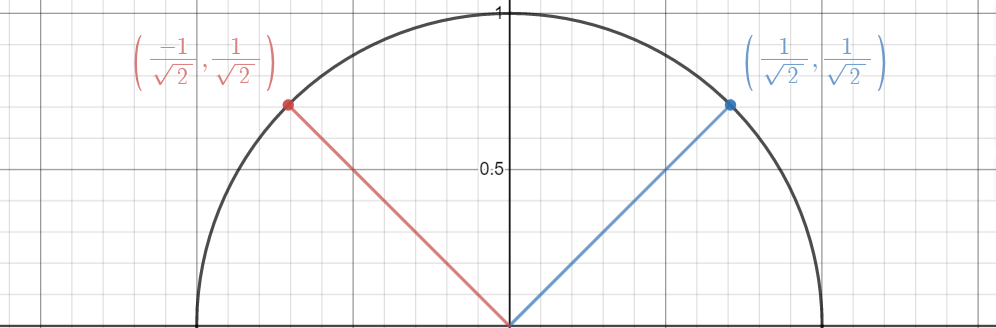
\includegraphics[width=\linewidth]{resources/img/orthonormal_bases_theta_pi_by_2.png}
				\caption{$ (\cos{\pi/4}, \sin{\pi/4})^T = (1/\sqrt{2}, 1/\sqrt{2})^T,\;  (-\sin{\pi/4}, \cos{\pi/4})^T = (-1/\sqrt{2}, 1/\sqrt{2})^T $}
			\end{figure}
			\\But for any value of the angle $\theta$ these remain orthogonal as can be seen if we generate the basis vectors for ${ \theta = \pi/3 }$.
			\begin{figure}[h!]
				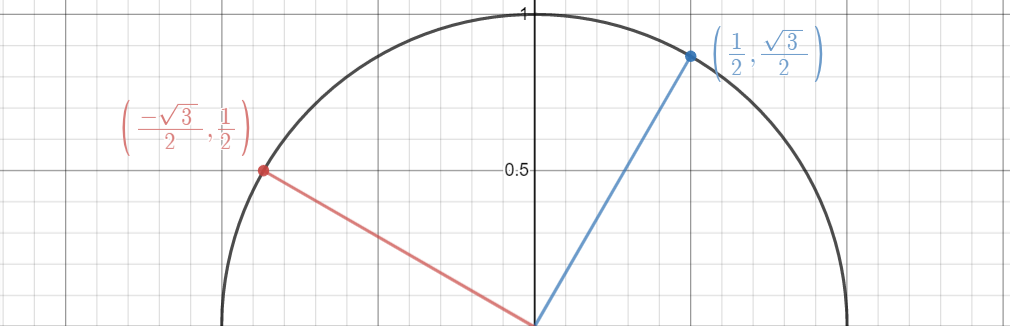
\includegraphics[width=\linewidth]{resources/img/orthonormal_bases_theta_pi_by_3.png}
				\caption{$ (\cos{\pi/3}, \sin{\pi/3})^T = (1/2, \sqrt{3}/2)^T,\;  (-\sin{\pi/3}, \cos{\pi/3})^T = (-\sqrt{3}/2, 1/2)^T $}
			\end{figure}
	
		
		\bigskip\bigskip
		\subsubsection{Orthogonal Operators}
		\bigskip
		\boxeddefinition{A matrix whose columns form an orthonormal basis is called an \textbf{orthogonal matrix}.\\\\
			The operation of left multiplication by such a matrix is called an \textbf{orthogonal operator}.
		}
	
		\medskip
		\labeledProposition{If a matrix $A$ is orthogonal then ${ A^T = \inv{A}}$.}{orthogonal_matrix_transpose_is_inverse}
		\begin{proof}
			$A$ is an orthogonal matrix so, by definition, its columns form an orthogonal basis. Then,
			\begin{align*}
			&& A^TA &=
					\begin{bmatrix}
						a_{11} & a_{21} & \cdots & a_{n1}\\
						a_{12} & a_{22} & \cdots & a_{n2}\\
						\vdots \\
						a_{1n} & a_{2n} & \cdots & a_{nn}
					\end{bmatrix}
					\begin{bmatrix}
						a_{11} & a_{12} & \cdots & a_{1n}\\
						a_{21} & a_{22} & \cdots & a_{2n}\\
						\vdots \\
						a_{n1} & a_{n2} & \cdots & a_{nn}
					\end{bmatrix} \\
			&&  &= \begin{bmatrix}
						a_{11}^2 + \cdots + a_{n1}^2 & a_{11}a_{12} + \cdots + a_{n1}a_{n2} & \cdots\\
						a_{12}a_{11} + \cdots + a_{n2}a_{n1} & a_{12}^2 + \cdots + a_{n2}^2 & \cdots\\
						\vdots \\
						\cdots & \cdots & \cdots & a_{1n}^2 + \cdots + a_{nn}^2
					\end{bmatrix}
			\end{align*}
			Along the main diagonal the components take the form
			\[ a_{1j}^2 + a_{2j}^2 + \cdots + a_{nj}^2 = a_j \dotprod a_j \]
			where ${ a_j }$ is the $j$th column of the matrix $A$. But the columns of $A$ are vectors in an orthonormal basis and so ${ a_j \dotprod a_j= 1 }$.\\
			Furthermore, the off-diagonal values take the form
			\[ a_{1j}a_{1j'} + \cdots + a_{nj}a_{nj'} = a_j \dotprod a_{j'} \]
			for ${ j \neq j' }$. Since the columns are from an orthonormal basis we know that ${ a_j \dotprod a_{j'} = 0 }$.\\
			Therefore the resultant matrix looks like,
			\[ A^TA = \begin{bmatrix}
						1 & 0 & \cdots & 0\\
						0 & 1 & \cdots & 0\\
						\vdots\\
						0 & 0 & \cdots & 1
					  \end{bmatrix}
					  = I_n.
			\]
			Clearly, the same effect would be seen for ${ AA^T }$ and so,
			\[ A^TA = AA^T = I \iff A^T = \inv{A}. \qedhere \]
		\end{proof}
	
		\bigskip
		\labeledProposition{Left multiplication by an orthogonal matrix preserves the dot product. In other words, for all vectors ${ \v,\w }$, $A$ is an orthogonal matrix if and only if,
			\[ A\v \dotprod A\w = \v\dotprod\w. \]
		}{left_mult_by_ortho_matrix_preserves_dot_product}
		\begin{proof}
			Using \autoref{prop:orthogonal_matrix_transpose_is_inverse} and the matrix formula for the dot product we can deduce that, for all vectors ${ \v,\w }$,
			\begin{align*}
			&& A\v \dotprod A\w &= (A\v)^T A\w \\
			&&  &= \v^TA^TA\w &\sidecomment{} \\
			&&  &= \v^T\w &\sidecomment{$A$ is orthogonal so ${A^TA = I}$} \\
			&&  &= \v \dotprod \w
			\end{align*}
			which is to say that an orthogonal matrix preserves the dot product.\\
			
			Conversely, if we assume that $A$ preserves the dot product then, for all vectors ${ \v,\w }$,
			\begin{align*}
			&& A\v \dotprod A\w &= \v \dotprod \w  \\
			&\iff & (A\v)^TA\w &= \v^T\w & \\
			&\iff & \v^TA^TA\w &= \v^T\w & \\
			&\iff & \v^TA^TA\w - \v^T\w &= 0 & \sidecomment{both terms are scalars}\\
			&\iff & \v^T(A^TA - I)\w &= 0. &
			\end{align*}
			Now for any arbitrary matrix $B$, 
			\[ e_i^TBe_j = b_{ij} \]
			where $b_{ij}$ is the $(i,j)$th element of $B$. Then, for
			\[ e_i^TBe_j = 0 \]
			to be true \textit{for all possible} ${ e_i,e_j }$ would require that, 
			\[ \forall i,j \logicsep b_{ij} = 0 \iff B = [0] \]
			where $[0]$ is the zero matrix. Therefore,
			\[ \forall \v,\w \logicsep \v^T(A^TA - I)\w = 0 \iff A^TA - I = [0] \iff A^TA = I \]
			and so if $A$ preserves the dot product then it is orthogonal.
		\end{proof}
	
	
		\bigskip
		\labeledProposition{The determinant of any orthogonal matrix is 1 or -1.}{determinant_of_orthogonal_matrix}
		\begin{proof}
			If a matrix $A$ is orthogonal then ${ A^TA = I }$ which implies that,
			\[ det(A^T)det(A) = det(I) = 1. \]
			By \autoref{prop:determinant_of_matrix_equal_to_its_transpose}, ${ det(A^T) = det(A) }$ so,
			\[ det(A^T)det(A) = det(A)^2 = 1 \iff \sqrt{det(A)} = 1 \iff det(A) = \pm 1.  \qedhere \]
		\end{proof}
	
		\note{If an orthogonal operator has determinant equal to 1 it is described as \textbf{orientation preserving} and if it is equal to -1 it is described as \textbf{orientation reversing}.}
		
		\bigskip
		\labeledProposition{The orthogonal matrices form a subgroup of $GL_n(\F{})$.}{orthogonal-matrices-are-subgroup}
		\begin{proof}
			Let ${ S = \setc{ A \in GL_n(\F{}) }{ A^TA = I } }$. Then,
			\begin{itemize}
				\item{$S$ is nonempty because ${ I \in S }$.}
				\item{For ${ B,C \in S }$,
					\[ (BC)^T(BC) = C^TB^T(BC) = C^T(B^TB)C = I \]
					so ${ BC \in S }$.
				}
				\item{For ${ B \in S }$, by \autoref{prop:orthogonal_matrix_transpose_is_inverse}, ${ \inv{B} = B^T }$ and
					\[ (B^T)^TB^T = BB^T = B\inv{B} = I \]
					so $S$ contains inverses.
				}
			\end{itemize}
			Therefore ${ S \leq GL_n(\F{}) }$.	
		\end{proof}
		
		\medskip
		\note{The subgroup of the general linear group formed by the orthogonal matrices is called the \textbf{orthogonal group} and is denoted $O_n$.}
	}


% --------------------


\pagebreak
\searchableSubsection{Linear and Affine Transformations}{linear algebra}{
	\bigskip\bigskip
	\subsubsection{Affine Spaces}
	\boxeddefinition{An \textbf{affine space} is a generalization of a Euclidean space in which there is no particular point designated as the origin. As a result vectors can be viewed as displacements rather than points.\\\\
		Let $V$ be a vector space and $P$ be a set of points. Then we can form an affine space over $V$ and $P$ by defining the vectors in $V$ as displacements connecting members of $P$ such that, for ${ Q_1,Q_2 \in P,\, \v \in V }$,
		\[ Q_1 + \v = Q_2 \iff Q_2 - Q_1 = \v \iff Q_1 - Q_2 = -\v. \]
	}
	\boxeddefinition{A \textbf{frame} of an affine space is an extension of a basis of its underlying vector space to include a point designated as an origin. If ${ \v_1,\dots,\v_n }$ is a basis of a vector space $V$ and $Q$ is a point in the set of points $P$, then ${ F = (\v_1,\dots,\v_n, Q) }$ is a frame of the affine space over $V$ and $P$.}
	\boxeddefinition{The \textbf{dimension} of an affine space is the dimension of the underlying vector space.}
	
	\bigskip
	\labeledProposition{Any linear combination of points in an affine space where the coefficients sum to 0 results in a vector.}{sum_affine_points_with_coeffs_sum_to_zero_are_vectors}
	\begin{proof}
		Let $S$ be a sum of $n$ points ${ Q_i \in P }$ in an affine space associated with a vector space $V$ such that,
		\[ S = \sum_{i=0}^n \alpha_i Q_i  \eqand \sum_{i=0}^n \alpha_i = 0. \]
		Then, if we take the partial sum of the first two points,
		\[ S_2 = \alpha_1 Q_1 + \alpha_2 Q_2 = \alpha_1(Q_1 - Q_2) + (\alpha_1 + \alpha_2)Q_2 \]
		and then the next partial sum of the first three points,
		\begin{align*}
		S_3 &= \alpha_1(Q_1 - Q_2) + (\alpha_1 + \alpha_2)Q_2 + \alpha_3 Q_3 \\
		&= \alpha_1(Q_1 - Q_2) +  (\alpha_1 + \alpha_2)(Q_2 - Q_3) +  (\alpha_1 + \alpha_2 + \alpha_3) Q_3
		\end{align*}
		we can see that, by induction, the $n$th sum is,
		\begin{align*}
		S &= \alpha_1(Q_1 - Q_2) \\
		&\hspace{20pt} + (\alpha_1 + \alpha_2)(Q_2 - Q_3)\\
		&\hspace{20pt} + (\alpha_1 + \alpha_2 + \alpha_3)(Q_3 - Q_4)\\
		&\hspace{24pt} \vdots\\
		&\hspace{20pt} + (\alpha_1 + \cdots + \alpha_{n-1})(Q_{n-1} - Q_n)\\
		&\hspace{20pt} + (\alpha_1 + \cdots + \alpha_n)Q_n.
		\end{align*}
		But we have ${ \alpha_1 + \cdots + \alpha_n = 0 }$ so the final term is 0. As a result $S$ is a summation of terms of the form,
		\[ (\alpha_1 + \cdots + \alpha_{i-1})(Q_{i-1} - Q_i) \]
		where ${ Q_{i-1} - Q_i }$ is a vector. Therefore $S$ is a linear combination of vectors in $V$ and is therefore also a vector in $V$.
	\end{proof}
	\begin{corollary}
		\label{coro:sum_affine_points_with_coeffs_sum_to_one_are_vectors}
		Any linear combination of points in an affine space where the coefficients sum to 1 results in a point.
	\end{corollary}
	\begin{proof}
		In the preceding proof if we had, instead, ${ \alpha_1 + \cdots + \alpha_n = 1 }$ then the final term would equal $Q_n$ and the resulting summation would be a vector plus the point $Q_n$. Therefore the sum is a point.
	\end{proof}

	\pagebreak
	\subsubsection{Intuition of Affine Spaces}
	\begin{wrapfigure}{l}{0.5\textwidth}
		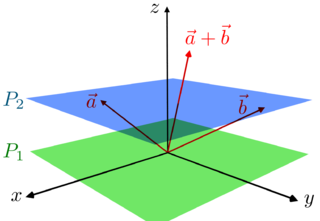
\includegraphics[width=0.9\linewidth]{resources/img/320px-Affine_space_R3.png} 
		\label{fig:affine_space_schematic}
	\end{wrapfigure}
	A translated linear subspace of a vector space like $P_2$ above that no longer passes through the origin is referred to as an \textbf{affine subspace}. It is not a vector space as ${ \0 \notin P_2 }$ and ${ \V{a},\V{b} \in P_2 }$ but ${ \V{a} + \V{b} \notin P_2 }$. 
	However, if we instead consider displacements between points --- e.g. ${ \V{b} - \V{a} }$ --- then we see the relationship between affine spaces and vector spaces: ${ \V{b} - \V{a} \in P_1 }$. The displacements between points in $P_2$ form a linear subspace. So we can define an affine space $A$ based on the set of points in $P_2$ and the vectors in $P_1$.
	

	\bigskip
	\subsubsection{Affine Combinations}
	\boxeddefinition{An \textbf{affine combination} of vectors is a combination such that the coefficients sum to 1.}
	\note{The definition of an affine combination differs from that of a convex combination in that the coefficients of a convex combination are additionally required to be non-negative.}
	
	\bigskip
	In an affine space there is no particular point designated as the origin but we can describe vector displacements between points as an ordered pair of points, for example, ${ (p,a) = \V{pa} }$. Affine combinations of displacements agree on the resulting point with linear combinations in the corresponding Euclidean space.\\
	For example, imagine a point $p$ in an affine space is at coordinates ${ (-1,4) }$ in the corresponding Euclidean space and similarly points $a$ and $b$ are at ${ (3,4) }$ and ${ (6,1) }$ respectively. Then, if we take an affine combination of the displacements to $a$ and $b$ the resulting point is independent of the chosen origin point.
%	\begin{wrapfigure}{l}{0.5\textwidth}
%		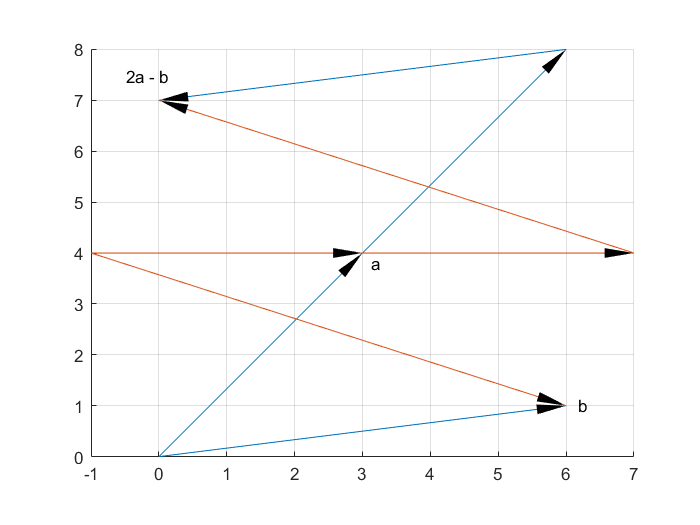
\includegraphics[width=\linewidth]{resources/img/affine_combinations_example.png} 
%		\label{fig:affine_combinations_example}
%	\end{wrapfigure}
%	
	
	\begin{figure}[h!]
		\centering
		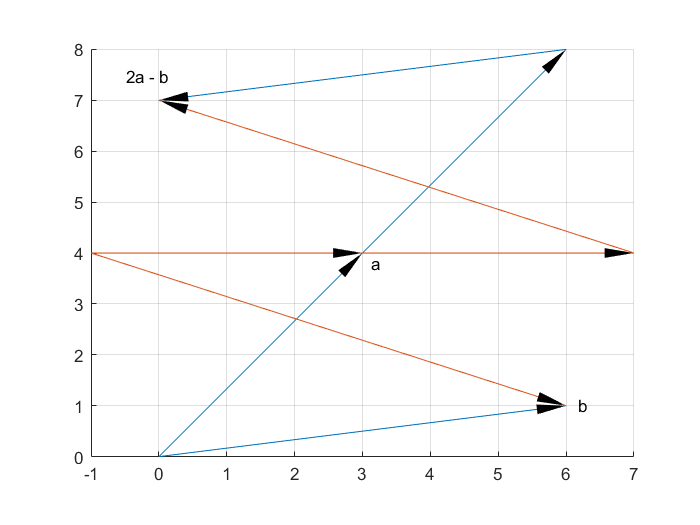
\includegraphics[width=300px]{resources/img/affine_combinations_example.png}
		\caption{\small The diagram shows the affine combination ${ 2\V{a} - \V{b} = 2\V{pa} - \V{pb} }$ where $\V{a}$ denotes the usual position vector in the Euclidean space.}
		\label{fig:affine_combinations_example}
	\end{figure}

	
	
	\bigskip\bigskip\bigskip
	\subsubsection{Affine Transformations}
	\boxeddefinition{Let ${ T: A_1 \longmapsto A_2 }$ be a mapping between the affine spaces $A_1$ and $A_2$. Then $T$ is an \textbf{affine transformation} if:
		\begin{itemize}
			\item{$T$ maps vectors to vectors and points to points.}
			\item{$T$ is a linear transformation over the vectors in the underlying vector space.}
			\item{${ T(Q + \v) = T(Q) + T(\v) }$.}
		\end{itemize}
	}

	\medskip
	\note{In an affine space a \textbf{translation} can be regarded as a change of frame in which we \textbf{change the origin point} while the vector basis may remain unchanged.}
	
	\medskip
	\labeledProposition{Affine transformations preserve parallelism.}{affine_transformations_preserve_parallelism}
	\begin{proof}
		Let $A$ be an affine space defined over a set of points $P$ and a vector space $V$ and let ${ Q_1,Q_2 \in P }$ and ${ \v \in V }$. Then, for ${ s,t \in \F{} }$,
		\[ l_1 = Q_1 + t\v \eqand l_2 = Q_2 + s\v \]
		are parallel lines in $A$. Let $T$ be an arbitrary affine transformation over $A$. Then,
		\[ l_1' = T(l_1) = T(Q_1) + tT(\v) \eqand l_2' = T(l_2) = T(Q_2) + sT(\v) \]
		are also parallel.
	\end{proof}

	\medskip
	\labeledProposition{An affine transformation that preserves the dot product is left multiplication by an orthogonal matrix.}{dot-product-preserving-affine-trans-is-left-mult-by-ortho-matrix}
	\begin{proof}
		Firstly, note that if a transformation $m$ preserves the dot product and also fixes the standard basis vectors $\e{i}$ then,
		\[ m(\e{i}) = \e{i} \eqand x_i = \x \dotprod \e{i} = m(\x) \dotprod m(\e{i}) = m(\x) \dotprod \e{i} = m(\x)_i. \]
		Therefore, such a transformation $m$ is the identity transformation.\\
		Now, assume a transformation $m'$ preserves the dot product (but does not necessarily fix the standard basis vectors) in $\R{n}$ and let 
		\[ B' = \{ m'(\e{1}),\dots,m'(\e{n}) \} \]
		be the transformed standard basis vectors. Then, if $[B']$ is the matrix whose columns are the elements of $B'$ then, because $m'$ preserves the dot product, $[B']$ is an orthogonal matrix as, by \autoref{prop:orthogonal-matrices-are-subgroup}, is $\inv{[B']}$. So, composing this with $m'$,
		\[ m'' = \inv{[B']}m' \]
		is a transformation that both preserves the dot product and fixes the standard basis vectors. Therefore we have,
		\[ m'' = I_n = \inv{[B']}m' \iff [B'] = m' \]
		so that $m'$ is left multiplication by $[B']$, an orthogonal matrix.
	\end{proof}

	\bigskip\bigskip
	\subsubsubsection{Properties of affine transformations}
	We can characterize affine transformations according to their form and behaviour in the Euclidean spaces $\R{2}$ and $\R{3}$. Specifically, whether the transformation:
	\begin{enumerate}
		\item{Fixes the origin: ${ T(\0) = \0 }$}
		\item{Preserves the dot product: ${ T(\v)\dotprod T(\w) = \v\dotprod\w }$, matrix is orthogonal}
		\item{Preserves distances: ${ \norm{T(\v) - T(\w)} = \norm{\v - \w} }$}
		\item{Preserves angles: matrix is scalar multiple of orthogonal matrix}		
		\item{Preserves orientation: transformation does not include a reflection, determinant of matrix is positive}
		\item{Preserves parallelism: transformation exhibits affine property (linearity under affine combinations)}
	\end{enumerate}

	As we can see here, the property of preserving parallelism depends only on the affine property so clearly, all affine transformations exhibit this behaviour. As a consequence of preserving parallelism, affine transformations preserve the dimension of affine subspaces (points, lines, planes, etc.). They do not preserve distances between points however, but they do preserve ratios of distances between points lying on a straight line.\\
	
	\bigskip
	\subsubsubsection{Classes of affine transformations}
	The most common subclassifications of affine transformations are:
	\begin{itemize}
		\item{Linear: preserves the origin.}
		\item{Conformal: preserves angles.}
		\item{Isometry (also known as a congruent transformation): preserves distances in metric spaces and so also implicity, angles. In a Euclidean space these transformations are known as a Euclidean isometries or rigid transformations.}
		\item{Rigid Motion: Euclidean isometry / rigid transformation that also preserves orientation.}
	\end{itemize}

	\bigskip
	\subsubsection{Isometries}
	\bigskip
	A Euclidean isometry or rigid motion, for example, carries a triangle to a congruent triangle. So, it preserves distances and angles but not necessarily orientation (a reflection flips the orientation).\\
	The composition of two rigid motions is a rigid motion and the inverse of a rigid motion is also a rigid motion. Therefore, the rigid motions of $\R{n}$ form a group under composition of operations. This group is called the \textit{group of motions} and denoted $M_n$.
	
	\bigskip
	\labeledProposition{A rigid motion that fixes the origin preserves the dot product.}{non-translational-isometries-preserve-dot-product}
	\begin{proof}
		Let $m$ be a rigid motion that fixes the origin. Then $m$ is an isometry and so preserves distances and also $m$ maps the origin to the origin. So we have,
		\[ \norm{m(\v) - m(\w)} = \norm{\v - \w} \eqand m(\0) = \0. \]
		We can rewrite the isometry property as,
		\begin{align*}
		&& \sqrt{(m(\v) - m(\w))\dotprod(m(\v) - m(\w))} &= \sqrt{(\v - \w)\dotprod(\v - \w)}\\
		&\iff & (m(\v) - m(\w))\dotprod(m(\v) - m(\w)) &= (\v - \w)\dotprod(\v - \w). &\sidecomment{}
		\end{align*}
		Now, if we take the case where ${ \w = \0 = m(\w) }$,
		\begin{align*}
		&& (m(\v) - \0)\dotprod(m(\v) - \0) &= (\v - \0)\dotprod(\v - \0) \\
		&\iff & m(\v) \dotprod m(\v) &= \v \dotprod \v. &\sidecomment{}
		\end{align*}
		and we can deduce that ${ m(\x) \dotprod m(\x) = \x \dotprod \x }$ for any vector $\x$. Using this along with the properties of the dot product we obtain,
		\begin{align*}
		&& (m(\v) - m(\w))\dotprod(m(\v) - m(\w)) &= (\v - \w)\dotprod(\v - \w) \\
		&\iff & m(\v)\dotprod m(\v) + m(\w)\dotprod m(\w) - 2m(\v)\dotprod m(\w) &= \v\dotprod\v + \w\dotprod\w - 2\v\dotprod\w &\sidecomment{} \\
		&\iff & -2m(\v)\dotprod m(\w) &= -2\v\dotprod\w &\sidecomment{} \\
		&\iff & m(\v)\dotprod m(\w) &= \v\dotprod\w. &\sidecomment{}
		\end{align*}
		
		Therefore, $m$ preserves the dot product and, by \autoref{prop:dot-product-preserving-affine-trans-is-left-mult-by-ortho-matrix}, is left multiplication by an orthogonal matrix.
	\end{proof}
	\begin{corollary}
		\label{coro:isometry-fixes-origin-left-mult-by-orthogonal-matrix}
		A rigid motion that fixes the origin is left multiplication by an orthogonal matrix and, therefore, also a linear operator.
	\end{corollary}

	\medskip
	\labeledProposition{Left multiplication by any orthogonal matrix is a Euclidean isometry (a rigid motion) that fixes the origin.}{left-mult-by-ortho-matrix-is-rigid-motion}
	\begin{proof}
		By, \autoref{prop:left_mult_by_ortho_matrix_preserves_dot_product}, left multiplication by an orthogonal matrix preserves the dot product. So, if $m$ is an affine transformation such that ${ m(\x) = A\x  }$ where $A$ is an orthogonal matrix then,
		\begin{align*}
		&& \norm{m(\v - \w)}^2 = m(\v - \w)\dotprod m(\v - \w) &= (\v - \w)\dotprod (\v - \w) = \norm{\v - \w}^2 \\
		&\iff & \norm{m(\v - \w)} &= \norm{\v - \w} &\sidecomment{} \\
		\end{align*}
		But also, left multiplication by a matrix is a linear operator so ${ m(\v - \w) = m(\v) - m(\w) }$ meaning that,
		\[ \norm{m(\v - \w)} = \norm{m(\v) - m(\w)} = \norm{\v - \w} \]
		which is the isometry property for $m$.
	\end{proof}
	
	
	\bigskip\bigskip
	\subsubsubsection{Linear}
	Isometries that fix the origin are linear operators and rigid motions in Euclidean space.\\
		
	
	\bigskip
	\subsubsubsection{Translation}
	If $T$ is a translation then, in general, ${ T(\0) \neq \0 }$ so translations do not fix the origin and, as a result, are \textbf{not} linear transformations. However, translations preserve distances and angles (and orientation because there is no reflection) so they are rigid motions. For example:
	\begin{exe}
		\ex{Let ${ \v = (v_1,\dots,v_n) }$ be any fixed vector in $\R{n}$. Then translation by $\v$ is the map,
			\[ t_v(\x) = \x + \v = \begin{bmatrix}x_1 + v_1\\\vdots\\x_n + v_n\end{bmatrix} \]
			which can be seen to be isometric (a rigid transformation) by,
			\begin{align*}
			&& t_v(\x) - t_v(\V{y}) = (\x + \v) - (\V{y} +\v) &= \x - \V{y} \\
			&\implies & \norm{t_v(\x) - t_v(\V{y})} &= \norm{\x - \V{y}}. &\sidecomment{}
			\end{align*}
		}
	\end{exe}

	\medskip
	\labeledProposition{Every rigid motion $m$ is the composition of an orthogonal linear operator and a translation. In other words, for some orthogonal matrix $A$ and fixed vector $\v$, it takes the form,
		\[ m(\x) = A\x + \v. \]
	}{every_rigid_motion_is_linear_op_plus_translation}
	\begin{proof}
		Let ${ \v = m(\0) }$ and ${ t_v(\x) = \x + \v }$ with inverse ${ t_{-v}(\x) = \x - \v }$. Then composing this with $m$, the resulting transformation,
		\[ (t_{-v} \circ m)(\x) = m(\x) - \v \]
		continues to be isometric --- because it is the composition of isometric transformations --- and it fixes the origin because ${ (t_{-v} \circ m)(\0) = m(\0) - \v = m(\0) - m(\0) = \0 }$. It is therefore, by \autoref{coro:isometry-fixes-origin-left-mult-by-orthogonal-matrix}, left multiplication by an orthogonal matrix. So we can represent it as,
		\[ (t_{-v} \circ m)(\x) = t_{-v}(m(\x)) = A\x. \]
		Since ${ t_{-v} = \inv{t_v} }$ we can apply $t_{v}$ to both sides of the equation,
		\[ m(\x) = t_{v}(A\x) = A\x + \v. \]
		The obtained representation is uniquely determined by $m$ as ${ \v = m(\0) }$ is clearly unique and then the translation $t_{-v}$ is uniquely determined by $\v$ and then ${ A = (t_{-v} \circ m) }$ is unique for a given $\v$ and $m$.
	\end{proof}

	\medskip\note{For a rigid motion ${ m(\x) = A\x + \v }$, $m$ is orientation-preserving if the matrix $A$ is orientation-preserving and orientation-reversing if $A$ is orientation-reversing.}
	
	\bigskip
	\subsubsubsection{Rotation}
	Rotations preserve distances, angles and orientation and so are rigid motions. Rotations also fix a vector which is known as the axis of rotation. If the axis of rotation contains the origin then they fix the origin and so are linear operators.
	
	\medskip
	\labeledTheorem{The rotations of $\R{2}$ and $\R{3}$ about the origin are the linear operators whose matrices with respect to the standard basis are orthogonal and have determinant 1.}{rotations-of-r2-r3-about-origin-are-ortho-mat-det-1}
	\begin{proof}
		A rotation about the origin $m$ involves rotating the standard basis vectors through an angle $\theta$. It is in the definition of this rotation that the image of the standard basis vectors continue to subtend the same angle, ${ \pi/2 }$. Therefore, the rotation must preserve angles. It is also part of the definition that the image under rotation is not scaled so the rotation must preserve distances and must be a congruent transformation. Since the axis of rotation passes through the origin the origin is unchanged by this rotation and so these rotations are rigid motions that fix the origin and have the form,
		\[ m(\x) = A\x \]
		where $A$ is an orthogonal matrix. Additionally, rotations do not change the orientation of an shape and so their matrices have determinant 1.
	\end{proof}

	\medskip
	\note{The rotation matrices --- orthogonal matrices with determinant 1 --- form a subgroup of the group $O_n$ of orthogonal matrices called the \textbf{special orthogonal group} and denoted $SO_n$.}
	
	\labeledProposition{Every member of the special orthogonal group ${ A \in SO_2 }$ is the matrix of a rotation.}{all-members-SO2-are-rotations}
	\begin{proof}
		Let ${ A \in SO_2 }$. Then $A$ is a ${ 2 \times 2 }$ orthogonal matrix with determinant 1. Let $\v_1$ be the first column of $A$ which, since $A$ is orthogonal, is a unit vector. Now assume that $R$ is the matrix of a rotation whose first column is $\v_1$ --- which is possible because $\v_1$ is a unit vector so $R$ can be orthogonal. Then the matrix
		\[ B = \inv{R}A \]
		fixes $\e{1}$ and also, as the composition of two orthogonal vectors, is orthogonal. Therefore the second column of $B$ is a unit vector orthogonal to $\e{1}$ which could be $\e{2}$ or $-\e{2}$. 
		
		However, $R$ is an orthogonal matrix with determinant 1 and so is a member of $SO_2$ which means that ${ \inv{R}A = B }$ is also in $SO_2$. 
		
		This, in turn, means that $B$ has determinant 1 which implies that the second column of $B$ is not $-\e{2}$ and is, therefore, $\e{2}$. So, we have obtained the result that ${ B = I = \inv{R}A }$ which implies that ${ R = A }$.
	\end{proof}

	\bigskip
	\subsubsubsection{Rotating $\bm{\R{2}}$ about the origin}
	Rotating the 2-d plane about the origin means that the axis of rotation is just the origin (so the fixed vector is $\0$).
	
	For example:
	\begin{exe}
		\ex{A rotation $\rho_{\theta}$ of the plane through an angle $\theta$ is a linear operator on $\R{2}$ whose matrix with respect to the standard basis is
			\[ R = 	\begin{bmatrix}
			\cos\theta & -\sin\theta\\
			\sin\theta & \cos\theta
			\end{bmatrix}.
			\]
			We can see that this is a rotation if we take ${ \x = (x_1,x_2)^T \in \R{2} }$ and write it in polar coordinates,
			\[ \x = (r,\alpha). \]
			So, relating the polar and rectangular coordinates,
			\[ \x = (r\cos\alpha, r\sin\alpha)^T. \]
			When we left-multiply by $R$,
			\begin{align*}
			R\x &= \begin{bmatrix}
			\cos\theta & -\sin\theta\\
			\sin\theta & \cos\theta
			\end{bmatrix}
			\begin{bmatrix}
			r\cos\alpha\\
			r\sin\alpha
			\end{bmatrix} \\
			&= \begin{bmatrix}
			r\cos\alpha\cos\theta - r\sin\alpha\sin\theta\\
			r\cos\alpha\sin\theta + r\sin\alpha\cos\theta
			\end{bmatrix} \\
			&= 	\begin{bmatrix}
			r\cos{(\alpha + \theta)}\\
			r\sin{(\alpha + \theta)}
			\end{bmatrix}.
			\end{align*}
			Note that $R$ is orthogonal because
			\[  \begin{bmatrix}
			\cos\theta\\
			\sin\theta
			\end{bmatrix} \dotprod 
			\begin{bmatrix}
			-\sin\theta\\
			\cos\theta
			\end{bmatrix} = -\cos\theta\sin\theta + \sin\theta\cos\theta = 0 \]
			and ${ det\,R = 1 }$,
			\[ 
			\begin{vmatrix}
			\cos\theta & -\sin\theta\\
			\sin\theta & \cos\theta
			\end{vmatrix} = \cos^2\theta + \sin^2\theta = 1.
			\]
		}
	\end{exe}

	\bigskip
	\subsubsubsection{Rotating $\bm{\R{3}}$ about the origin}	 
	\boxeddefinition{Define $\rho$ as a rotation in $\R{3}$ around the origin if:
	\begin{enumerate}[label=(\roman*)]
		\item{$\rho$ is a rigid motion (orientation-preserving Euclidean isometry) that fixes the origin;}
		\item{$\rho$ also fixes a nonzero vector $\v$;}
		\item{$\rho$ operates as a rotation on the plane $P$ orthogonal to $\v$.}
	\end{enumerate}}
	\note{Note that this definition could be described as selecting a 2-dimensional subspace of $\R{3}$ and performing a 2-dimensional rotation on it as if it were $\R{2}$.}
	Condition (i) implies, by \autoref{coro:isometry-fixes-origin-left-mult-by-orthogonal-matrix}, that $\rho$ is left multiplication by an orthogonal matrix. Condition (ii) states that $\rho$ has an eigenvector $\v$ with eigenvalue 1. Then, because $\rho$ preserves angles, the plane $P$ referenced in condition (iii) that is orthogonal to the eigenvector $\v$, must map to a plane that is orthogonal to the map of $\v$ in the image of $\rho$. But $\v$ is fixed by $\rho$ and is unchanged in the image. Also $\v$ uniquely identifies a plane orthogonal to it. Therefore the plane $P$ is unchanged in the image also. In other words, $P$ is an invariant subspace. So, condition (iii) says that the restriction of $\rho$ to this invariant subspace is a rotation.
	
	\bigskip
	For example:
	\begin{exe}
		\ex{A rotation of $\R{3}$ about the origin can be described by a pair $(\v, \theta)$ consisting of a unit
			vector $\v$, a vector of length 1, which lies in the axis of rotation, and a nonzero angle
			$\theta$, the angle of rotation. The two pairs $(\v, \theta)$ and $(-\v, -\theta)$ represent the same rotation.
			We also consider the identity map to be a rotation, though its axis is indeterminate.\\
			The matrix representing a rotation through the angle $\theta$ about the vector $\e{1}$ is obtained easily from the $2 \times 2$ rotation matrix. It is
			\[ A = \begin{bmatrix}
					1 & 0 & 0\\
					0 & \cos\theta & -\sin\theta\\
					0 & \sin\theta & \cos\theta
					\end{bmatrix}.
			\]
			Multiplication by $A$ fixes the first coordinate $x_1$ of a vector and operates by rotation on $(x_2, x_3)^T$. All rotations of $\R{3}$ are linear operators, but their matrices can be fairly complicated.
		}
	\end{exe}

	\bigskip
	\labeledProposition{Every element of $SO_3$ has eigenvalue 1.}{elements-of-SO3-have-eigenvalue-1}
	\begin{proof}
		Let ${ A \in SO_3 }$. Then $A$ is an orthogonal ${ 3 \times 3 }$ matrix with determinant equal to 1. Reasoning from orthogonality of $A$ we have,
		\begin{align*}
		&& A^TA &= I \\
		&\iff & A^TA - A^T &= I - A^T &\sidecomment{} \\
		&\iff & A^T(A - I) &= I - A^T &\sidecomment{} \\
		&\iff & A^T(A - I) &= (I - A)^T. &\sidecomment{by \autoref{prop:matrix-transpose-distributes-over-addition}}
		\end{align*}
		If we take the determinants of both sides of this equation we obtain,
		\begin{align*}
		&& det(A^T)\cdot det(A - I) &= det((I-A)^T) &\sidecomment{by \autoref{prop:determinant_of_matrix_product}} \\
		&\iff & det(A)\cdot det(A - I) &= det(I - A) &\sidecomment{by \autoref{prop:determinant_of_matrix_equal_to_its_transpose}} \\
		&\iff & det(A - I) &= det(I - A). &\sidecomment{${ det(A) = 1 }$}
		\end{align*}
		But the dimension of $A$ being 3 implies that
		\[ det(-A) = (-1)^3 det(A) = -det(A) \]
		so that,
		\[ det(A - I) = det(I - A) \iff det(A - I) = 0. \]
		Therefore $A$ has the eigenvalue 1.
	\end{proof}

	\bigskip
	\labeledProposition{The elements of $SO_3$ are precisely the rotations about the origin of $\R{3}$.}{elements-of-SO3-are-the-rotations-around-origin-in-R3}
	\begin{proof}
		Let ${ \rho: \R{3} \longmapsto \R{3} }$ be defined as ${ \rho(\x) = A\x }$ where ${ A \in SO_3 }$. Then,
		\begin{itemize}
			\item{by \autoref{prop:left-mult-by-ortho-matrix-is-rigid-motion} and orthogonality of ${ A \in SO_3 }$, left multiplication by $A$ is a rigid motion that fixes the origin. So $\rho$ is isometric and fixes the origin;}
			\item{\autoref{prop:elements-of-SO3-have-eigenvalue-1} shows that every ${ A \in SO_3 }$ has eigenvalue 1 which implies that $\rho$ fixes a nonzero vector;}
			\item{if we let $\v$ be the nonzero vector fixed by $\rho$ (i.e. its eigenvector with eigenvalue 1), then we can normalize it to find the unit vector parallel to $\v$, say $\u_1$. Next we can find two unit vectors orthogonal to $\u_1$ --- say $\u_2$ and $\u_3$ --- and these must be a basis for the plane orthogonal to $\v$. Furthermore, if we select $\u_2$ and $\u_3$ to be orthogonal to each other than ${ B = \{\u_1,\u_2,\u_3\} }$ is an orthonormal basis of $\R{3}$.\\
				Now if we define ${ P = \inv{[B]} }$ then,
				\[ A' = \inv{P}AP \]
				is similar to the matrix $A$ and so has the same determinant, 1. Furthermore, because $B$ is an orthonormal basis, the matrices ${ [B],\, \inv{[B]} = P }$ are orthogonal. Since both $P$ and $A$ are orthogonal, ${ \inv{P}AP = A' }$ is orthogonal also. Since $A'$ is orthogonal and has determinant equal to 1, it is a member of $SO_3$.\\
				If we examine the structure of $A'$, we see that the first column of $A'$ is $\v_1$ --- the unit vector in the direction of $\v$. Since $\v$ is an eigenvector of $\rho$ with eigenvalue 1, the first column of $A'$ is $\e{1}$ and since $A'$ is orthogonal, the other columns are orthogonal to the first. So the block structure of $A'$ looks like,
				\[ A' = \begin{bmatrix}
						1 & 0 \\
						0 & R
						\end{bmatrix} 
				\]
				where $R$ is a ${ 2 \times 2 }$ matrix.\\
				We know that the determinant of $A'$ is 1 and this implies that the determinant of $R$ is also 1. Furthermore, $R$ must also be orthogonal and so ${ R \in SO_2 }$. So, by \autoref{prop:all-members-SO2-are-rotations}, $R$ is a rotation. Therefore $R$ represents a rotation of the plane orthogonal to $\v$ and this implies that $\rho$ rotates the plane orthogonal to $\v$ as required.
			}
		\end{itemize}
	\end{proof}
	
	\bigskip
	\subsubsubsection{Uniform Scaling}
	Uniform scaling is a scalar multiple of an orthogonal matrix and is therefore a linear operator which means that it fixes the origin. It also preserves angles but not distances between points.
	
	
	\bigskip\bigskip
	\subsubsection{Conformal Transformations}
	\bigskip
	\subsubsubsection{Non-uniform Scaling}
	Non-uniform scaling, however, its matrix is not a scalar multiple of an orthogonal matrix and, as such, it does not preserve angles. An important example is:
	\begin{exe}
		\ex{\textbf{Mercator projection}:\\\\
			This is a map projection that was designed so that rhumb lines (lines of constant bearing over the surface of the earth) are straight lines on the map. To achieve this the projection ensures that a square on the surface of the earth presents as a square on the map.\\
			Then, modelling the earth as a sphere of radius $R$, if lines of latitude are horizontal grid lines across the map, then each actual line of latitude with circumference ${ 2\pi R \cos\phi }$ where $\phi$ is the angle of latitude will present on the map as the same length as the equator, which in reality is ${ 2\pi R }$. So they appear to be a line of length ${ \cos\phi }$ times longer than they actually are, i.e. they are stretched by ${ \sec{\phi} }$.\\
			So, the map projection will stretch the width of a square on the surface of the earth by ${ \sec{\phi} }$ and to maintain it as a square, it is necessary to stretch the height of the square by the same amount, ${ \sec{\phi} }$. The actual square on the surface of the earth has height (approximately for a small square) ${ R\Delta\phi }$ so, on the map we need a height ${ \Delta y \propto \Delta\phi\sec\phi }$. Therefore, we have,
			\[ \frac{dy}{d\phi} = \sec\phi \implies y = \ln{(\tan\phi + \sec\phi)} + c \]
			where $c$ is a constant that we can set to 0. 
			See \url{https://www.math.ubc.ca/~israel/m103/mercator/mercator.html} for a description of this derivation. For more information on conformal map projections generally see: \href{https://arxiv.org/pdf/1412.7690.pdf}{Map Projection, York University, Toronto} and \href{http://diposit.ub.edu/dspace/bitstream/2445/121898/2/memoria.pdf}{Conformal Cartographic
				Representations - University of Barcelona}.
		}
	\end{exe}
	
	\subsubsubsection{Reflection}
	Reflection usually refers to a Euclidean Isometry (rigid transformation over a Euclidean space) that fixes a hyperplane (so a line in $\R{2}$ and a plane in $\R{3}$) but does not preserve orientation so is not a rigid motion. However, it may also refer to a transformation that fixes an affine space of lower dimension than a hyperplane --- for example, reflection in a point --- in which case it does preserve orientation and is, therefore, a rigid motion (in fact, reflection in the origin in $\R{2}$ is equal to rotation by $\pi$). Reflection may fix the origin or may not, depending on whether or not the origin is contained in the affine space fixed by the reflection.
	
	\bigskip
	\subsubsection{Non-Rigid non-Conformal Transformations}
	\bigskip
	\subsubsubsection{Shear}
	Shear neither preserves distances nor angles. It does preserve parallelism though (as do all affine transformations) and it also fixes the origin, so it is a linear operator.
	
	\bigskip\bigskip
	\note{For more in-depth treatment of affine spaces and transformations see:
		\begin{itemize}
			\item{First two lectures of \href{https://web.ma.utexas.edu/users/dafr/M375T/}{University of Texas - Multivariable Analysis}.}
			\item{\url{https://www.maa.org/sites/default/files/pdf/pubs/books/meg/meg_ch12.pdf}}
		\end{itemize}
	}
}	

\end{document}